    
%%%%%%%%%%%%%%%%%%%%%%%%%%%%%%%%%%%%%%%%%
% Short Sectioned Assignment LaTeX Template Version 1.0 (5/5/12)
% This template has been downloaded from: http://www.LaTeXTemplates.com
% Original author:  Frits Wenneker (http://www.howtotex.com)
% License: CC BY-NC-SA 3.0 (http://creativecommons.org/licenses/by-nc-sa/3.0/)
%%%%%%%%%%%%%%%%%%%%%%%%%%%%%%%%%%%%%%%%%

% \documentclass[paper=a4, fontsize=11pt]{scrartcl} % A4 paper and 11pt font size
\documentclass[11pt, a4paper]{book}
\usepackage[T1]{fontenc} % Use 8-bit encoding that has 256 glyphs
\usepackage[utf8]{inputenc}
%\usepackage{fourier} % Use the Adobe Utopia font for the document - comment this line to return to the LaTeX default
\usepackage{listings} % para insertar código con formato similar al editor
\usepackage[spanish, es-tabla]{babel} % Selecciona el español para palabras introducidas automáticamente, p.ej. "septiembre" en la fecha y especifica que se use la palabra Tabla en vez de Cuadro
\usepackage{url} % ,href} %para incluir URLs e hipervínculos dentro del texto (aunque hay que instalar href)
\usepackage{graphics,graphicx, float} %para incluir imágenes y colocarlas
\usepackage[gen]{eurosym} %para incluir el símbolo del euro
\usepackage{cite} %para incluir citas del archivo <nombre>.bib
\usepackage{lscape}
\usepackage{color}

\definecolor{dkgreen}{rgb}{0,0.6,0}
\definecolor{gray}{rgb}{0.5,0.5,0.5}
\definecolor{mauve}{rgb}{0.58,0,0.82}

\lstset{frame=tb,
  language=Java,
  aboveskip=3mm,
  belowskip=3mm,
  showstringspaces=false,
  columns=flexible,
  basicstyle={\small\ttfamily},
  numbers=none,
  numberstyle=\tiny\color{gray},
  keywordstyle=\color{blue},
  commentstyle=\color{dkgreen},
  stringstyle=\color{mauve},
  breaklines=true,
  breakatwhitespace=true,
  tabsize=3
}



% \documentclass[a4paper,11pt]{book}
% %\documentclass[a4paper,twoside,11pt,titlepage]{book}
% \usepackage{listings}
% \usepackage[utf8]{inputenc}
% \usepackage[spanish]{babel}
% \usepackage{graphics,graphicx, float} %para incluir imágenes y colocarlas

% \usepackage[style=list, number=none]{glossary} %
%\usepackage{titlesec}
%\usepackage{pailatino}

\decimalpoint
\usepackage{dcolumn}
\newcolumntype{.}{D{.}{\esperiod}{-1}}
\makeatletter
\addto\shorthandsspanish{\let\esperiod\es@period@code}
\makeatother


%\usepackage[chapter]{algorithm}
\RequirePackage{verbatim}
%\RequirePackage[Glenn]{fncychap}
\usepackage{fancyhdr}
\usepackage{graphicx}
\usepackage{afterpage}

\usepackage{longtable}

\usepackage[pdfborder={000}]{hyperref} %referencia

% ********************************************************************
% Re-usable information
% ********************************************************************
\newcommand{\myTitle}{Desarrollo de un test de condición física mediante plataforma móvil\xspace}
\newcommand{\myDegree}{Grado en Ingeniería Informática\xspace}
\newcommand{\myName}{José Luis López Sánchez\xspace}
\newcommand{\myProf}{Raquel ureña (tutor1)\xspace}
\newcommand{\myOtherProf}{Enrique Herrera Viedma\xspace}
%\newcommand{\mySupervisor}{Put name here\xspace}
\newcommand{\myFaculty}{Escuela Técnica Superior de Ingenierías Informática y de
Telecomunicación\xspace}
\newcommand{\myFacultyShort}{E.T.S. de Ingenierías Informática y de
Telecomunicación\xspace}
\newcommand{\myDepartment}{Departamento de Ciencias de la Computación e Inteligencia Artificial\xspace}
\newcommand{\myUni}{\protect{Universidad de Granada}\xspace}
\newcommand{\myLocation}{Granada\xspace}
\newcommand{\myTime}{\today\xspace}
\newcommand{\myVersion}{Version 0.1\xspace}


\hypersetup{
pdfauthor = {\myName (lopezjoseluis (en) correougr (punto) es)},
pdftitle = {\myTitle},
pdfsubject = {},
pdfkeywords = {android, app, java, acelerómetro, salud, Short Physical Battery Test, SPPB, condición física, base de datos},
pdfcreator = {LaTeX con el paquete ....},
pdfproducer = {pdflatex}
}

%\hyphenation{}


%\usepackage{doxygen/doxygen}
%\usepackage{pdfpages}
\usepackage{url}
\usepackage{colortbl,longtable}
\usepackage[stable]{footmisc}
%\usepackage{index}

%\makeindex
%\usepackage[style=long, cols=2,border=plain,toc=true,number=none]{glossary}
% \makeglossary

% Definición de comandos que me son tiles:
%\renewcommand{\indexname}{Índice alfabético}
%\renewcommand{\glossaryname}{Glosario}

\pagestyle{fancy}
\fancyhf{}
\fancyhead[LO]{\leftmark}
\fancyhead[RE]{\rightmark}
\fancyhead[RO,LE]{\textbf{\thepage}}
\renewcommand{\chaptermark}[1]{\markboth{\textbf{#1}}{}}
\renewcommand{\sectionmark}[1]{\markright{\textbf{\thesection. #1}}}

\setlength{\headheight}{1.5\headheight}

\newcommand{\HRule}{\rule{\linewidth}{0.5mm}}
%Definimos los tipos teorema, ejemplo y definición podremos usar estos tipos
%simplemente poniendo \begin{teorema} \end{teorema} ...
\newtheorem{teorema}{Teorema}[chapter]
\newtheorem{ejemplo}{Ejemplo}[chapter]
\newtheorem{definicion}{Definición}[chapter]

\definecolor{gray97}{gray}{.97}
\definecolor{gray75}{gray}{.75}
\definecolor{gray45}{gray}{.45}
\definecolor{gray30}{gray}{.94}

\lstset{ frame=Ltb,
     framerule=0.5pt,
     aboveskip=0.5cm,
     framextopmargin=3pt,
     framexbottommargin=3pt,
     framexleftmargin=0.1cm,
     framesep=0pt,
     rulesep=.4pt,
     backgroundcolor=\color{gray97},
     rulesepcolor=\color{black},
     %
     stringstyle=\ttfamily,
     showstringspaces = false,
     basicstyle=\scriptsize\ttfamily,
     commentstyle=\color{gray45},
     keywordstyle=\bfseries,
     %
     numbers=left,
     numbersep=6pt,
     numberstyle=\tiny,
     numberfirstline = false,
     breaklines=true,
   }
 
% minimizar fragmentado de listados
\lstnewenvironment{listing}[1][]
   {\lstset{#1}\pagebreak[0]}{\pagebreak[0]}

\lstdefinestyle{CodigoC}
   {
	basicstyle=\scriptsize,
	frame=single,
	language=C,
	numbers=left
   }
\lstdefinestyle{CodigoC++}
   {
	basicstyle=\small,
	frame=single,
	backgroundcolor=\color{gray30},
	language=C++,
	numbers=left
   }

 
\lstdefinestyle{Consola}
   {basicstyle=\scriptsize\bf\ttfamily,
    backgroundcolor=\color{gray30},
    frame=single,
    numbers=none
   }


\newcommand{\bigrule}{\titlerule[0.5mm]}


%Para conseguir que en las páginas en blanco no ponga cabecerass
\makeatletter
\def\clearpage{%
  \ifvmode
    \ifnum \@dbltopnum =\m@ne
      \ifdim \pagetotal <\topskip
        \hbox{}
      \fi
    \fi
  \fi
  \newpage
  \thispagestyle{empty}
  \write\m@ne{}
  \vbox{}
  \penalty -\@Mi
}
\makeatother

\usepackage{pdfpages}
\begin{document}
\begin{titlepage}
 
 
\newlength{\centeroffset}
\setlength{\centeroffset}{-0.5\oddsidemargin}
\addtolength{\centeroffset}{0.5\evensidemargin}
\thispagestyle{empty}

\noindent\hspace*{\centeroffset}\begin{minipage}{\textwidth}

\centering

\includegraphics[width=0.9\textwidth]{imagenes/logo_ugr.jpg}\\[1cm]

\textsc{ \Large TRABAJO FIN DE GRADO\\[0.2cm]}
\textsc{ INGENIERÍA EN INFORMÁTICA}\\[1.4cm]
% Upper part of the page
% 
% Title
{\Huge\bfseries Desarrollo de un test de condición física mediante plataforma móvil\\
}
\noindent\rule[-1ex]{\textwidth}{3pt}\\[3.5ex]
%{\large\bfseries Subtitulo del Proyecto}
\end{minipage}

\vspace{2cm}
\noindent\hspace*{\centeroffset}\begin{minipage}{\textwidth}
\centering

\textbf{Autor}\\ {José Luis López Sánchez}\\[2.5ex]
\textbf{Directores}\\
{Raquel Ureña\\
Enrique Herrera Viedma}\\[2cm]

\includegraphics[width=0.3\textwidth]{imagenes/etsiit_logo.png}\\[0.1cm]
\textsc{Escuela Técnica Superior de Ingenierías Informática y de Telecomunicación}\\
\textsc{---}\\
Granada, septiembre de 2019
\end{minipage}
%\addtolength{\textwidth}{\centeroffset}
%\vspace{\stretch{2}}
\end{titlepage}



\chapter*{}
%\thispagestyle{empty}
%\cleardoublepage

%\thispagestyle{empty}

\begin{titlepage}
 
 
\setlength{\centeroffset}{-0.5\oddsidemargin}
\addtolength{\centeroffset}{0.5\evensidemargin}
\thispagestyle{empty}

\noindent\hspace*{\centeroffset}\begin{minipage}{\textwidth}

\centering
%
\includegraphics[width=0.9\textwidth]{imagenes/logo_ugr.jpg}\\[1.4cm]

%\textsc{ \Large PROYECTO FIN DE CARRERA\\[0.2cm]}
%\textsc{ INGENIERÍA EN INFORMÁTICA}\\[1cm]
% Upper part of the page
% 

 \vspace{3.3cm}

%si el proyecto tiene logo poner aquí

\includegraphics{imagenes/icon_small.png} 
 \vspace{0.5cm}

% Title

{\Huge\bfseries Desarrollo de un test de condición física mediante plataforma móvil\\
}
\noindent\rule[-1ex]{\textwidth}{3pt}\\[3.5ex]
%{\large\bfseries Subtítulo del proyecto.\\[4cm]}
\end{minipage}

\vspace{2.5cm}
\noindent\hspace*{\centeroffset}\begin{minipage}{\textwidth}
\centering

\textbf{Autor}\\ {José Luis López Sánchez}\\[2.5ex]
\textbf{Directores}\\
{Raquel Ureña\\
Enrique Herrera Viedma}\\[2cm]
%
\includegraphics[width=0.15\textwidth]{imagenes/tstc.png}\\[0.1cm]
%\textsc{Departamento de Teoría de la Señal, Telemática y Comunicaciones}\\
%\textsc{---}\\
%Granada, mes de 201
\end{minipage}
%\addtolength{\textwidth}{\centeroffset}
\vspace{\stretch{2}}

 
\end{titlepage}






\cleardoublepage
\thispagestyle{empty}

\begin{center}
{\large\bfseries Desarrollo de un test de condición física mediante plataforma móvil}\\
\end{center}
\begin{center}
José Luis López Sánchez\\
\end{center}

%\vspace{0.7cm}
\noindent{\textbf{Palabras clave}: android, app, java, acelerómetro, salud, Short Physical
Battery Test, SPPB, condición física, base de datos, fragilidad}\\

\vspace{0.7cm}
\noindent{\textbf{Resumen}}\\

Este proyecto consiste en el desarrollo de una aplicación móvil dirigida a la plataforma Android, que permitirá calcular la condición física de cualquier persona, especialmente de adultos mayores.

Para ello, se implementará un test conocido como "Batería reducida para la valoración del rendimiento físico", o SPPB por sus siglas en inglés, que cuenta con tres pruebas distintas: equilibrio, velocidad y levantarse repetidamente de una silla. 

La detección y medición del desarrollo de la prueba se llevará a cabo utilizando uno de los sensores de los que disponen los teléfonos actuales, en este caso el acelerómetro. El usuario podrá olvidarse de medir el tiempo que invierte en cada prueba, así como el número de repeticiones o la velocidad, centrándose exclusivamente en ejecutar las instrucciones correctamente. Esta será por tanto la característica diferenciadora del proyecto.

Habrá también una sección donde el usuario pueda guardar los resultados de cada prueba bajo el nombre que elija, datos que serán almacenados en una base de datos local para poder ser consultada posteriormente.

Como hemos mencionado anteriormente, la aplicación estará especialmente orientada a adultos mayores/ancianos, con lo que la interfaz debe de ser lo más intuitiva y sencilla posible, el tamaño de fuente de los textos ha de ajustarse a las preferencias establecidas en el dispositivo y los pasos para la ejecución de las pruebas deben ser claros y fáciles de entender.

En esta documentación trataremos además asuntos como el envejecimiento de la población, qué es la fragilidad, detección de la misma y consecuencias. También hablaremos sobre la plataforma Android y describiremos brevemente el funcionamiento del sistema operativo y su distribución o fragmentación. Por último, analizaremos los actores, requisitos, tecnologías, diseño y planificación que facilitarán el camino para la implementación y desarrollo de la aplicación final.
\cleardoublepage


\thispagestyle{empty}


\begin{center}
{\large\bfseries Development of a fitness test through mobile platform}\\
\end{center}
\begin{center}
Jose Luis López Sánchez\\
\end{center}

%\vspace{0.7cm}
\noindent{\textbf{Keywords}:  android, app, java, accelerometer, health, Short Physical
Battery Test, SPPB, physical condition, database, fragility}\\

\vspace{0.7cm}
\noindent{\textbf{Abstract}}\\

This project involves the development of a mobile application aimed at the Android platform, which will allow the calculation of the physical condition of any person, especially older adults.

To do this, a test known as "Short Physical Battery Test", or SPPB for its acronym, which has three different tests: balance, speed and repeatedly getting up from a chair.

The detection and measurement of the test development will be carried out using one of the sensors available on current phones, in this case the accelerometer. The user can forget about measuring the time spent in each test, as well as the number of repetitions or speed, focusing exclusively on executing the instructions correctly. This will therefore be the distinguishing feature of the project.

There will also be a section where the user can save the results of each test under the name he chooses, data that will be stored in a local database for later reference.

As we mentioned above, the application will be especially aimed at older adults / elders, so the interface must be as intuitive and simple as possible, the font size of the texts must conform to the preferences established in the device and the steps for the execution of the tests should be clear and easy to understand.

In this documentation we will also discuss issues such as the aging of the population, what is fragility, its detection and consequences. We also talk about the Android platform and briefly describe how the operating system works and its distribution or fragmentation. Finally, we will analyze the actors, requirements, technologies, design and planning that will facilitate the path for the implementation and development of the final application.

\chapter*{}
\thispagestyle{empty}

\noindent\rule[-1ex]{\textwidth}{2pt}\\[4.5ex]

Yo, \textbf{José Luis López Sánchez}, alumno de la titulación INGENIERÍA INFORMÁTICA de la \textbf{Escuela Técnica Superior
de Ingenierías Informática y de Telecomunicación de la Universidad de Granada}, con DNI 77392285E, autorizo la
ubicación de la siguiente copia de mi Trabajo Fin de Grado en la biblioteca del centro para que pueda ser
consultada por las personas que lo deseen.

\vspace{6cm}

\noindent Fdo: José Luis López Sánchez

\vspace{2cm}

\begin{flushright}
Granada a 22 de agosto de 2019.
\end{flushright}


\chapter*{}
\thispagestyle{empty}

\noindent\rule[-1ex]{\textwidth}{2pt}\\[4.5ex]

Dña. \textbf{Raquel Ureña}, Institute of Artificial Intelligence, De Montfort University Leicester, UK.

\vspace{0.5cm}

D. \textbf{Enrique Herrera Viedma}, Vicerrector de Investigación y Transferencia de la Universidad de Granada.


\vspace{0.5cm}

\textbf{Informan:}

\vspace{0.5cm}

Que el presente trabajo, titulado \textit{\textbf{Desarrollo de un test de condición física mediante plataforma móvil}}, ha sido realizado bajo su supervisión por \textbf{José Luis López Sánchez}, y autorizamos la defensa de dicho trabajo ante el tribunal
que corresponda.

\vspace{0.5cm}

Y para que conste, expiden y firman el presente informe en Granada a 2 de Septiembre de 2019.

\vspace{1cm}

\textbf{Los directores:}

\vspace{5cm}

\noindent \textbf{Raquel Ureña \ \ \ \ \ Enrique Herrera Viedma}

\chapter*{Agradecimientos}
\thispagestyle{empty}

       \vspace{1cm}


Este proyecto no es más que el broche final al trabajo realizado durante dos décadas para conseguir la formación de la que ahora dispongo, y en la que decenas o incluso cientos de personas han contribuido. No estaría aquí sin los valores, conocimientos y experiencias de incalculable valor que me han transmitido todos los profesores que tuve en todas y cada una de las etapas académicas que he atravesado. Me llevo un bonito recuerdo de cada uno, y espero algún día poder contribuir a la sociedad de la misma forma que ellos lo han hecho.

Gracias a todos esos profesores de la carrera que se implican al máximo en su trabajo, y que con su dedicación y compromiso, están formando auténticos profesionales. Nada de esto sería posible sin los conocimientos adquiridos estos últimos cuatro años.

Mil gracias a los amigos que he conocido en la carrera. Personas increíbles que han hecho fáciles los momentos difíciles, alegres los tristes y amenos los aburridos. Sé que las tardes de estudio habrían sido mucho más largas sin vuestras bromas, los exámenes mucho más difíciles sin vuestras explicaciones y las fiestas mucho más vacías sin vosotros. Os habéis convertido en la mejor parte de la mejor etapa.

Y como no podía ser de otro modo, un millón de gracias a mi pareja Marta, mi madre Virtudes, mi padre José Antonio, toda mi familia y mis amigos de siempre por aguantarme todos estos años, en los buenos momentos y (sobre todo) en los malos. Por creer siempre en mí y apoyarme. Por hacérmelo más fácil. Esta carrera es en parte de todos vosotros. 


\frontmatter
\tableofcontents
\listoffigures
%\listoftables

\mainmatter
\setlength{\parskip}{5pt}

\chapter{Introducción}

\section{Contextualización del trabajo y motivación}

Nos encontramos imbuidos en una constante y cada vez más acelerada revolución tecnológica. Ni siquiera han pasado cien años desde la invención del primer ordenador en 1936, llamado Z1, a manos de Honrad Zuse. Mucho más reciente es, sin embargo, su salto al mercado de consumo empujado por IBM, para el que tenemos que remontarnos a 1981\cite{primer_ordenador}. 

Con esto, la tecnología comenzó su entrada en muchos hogares de todo el mundo, lo que no evitó el asombro que produjo la llegada (1973) y popularización (en los años ochenta) de los primeros teléfonos móviles de mano de Motorola\cite{primer_movil}.

La unificación de estas dos invenciones tuvo lugar en 1992 con la presentación por parte de IBM del primer teléfono inteligente, al que denominaron Simon\cite{smartphone}. Contaba con calendario, libreta de notas, correo electrónico, FAX y calculadora entre otros. Hoy sería sin duda catalogado como un teléfono de gama baja, pero señaló el camino para todas las marcas y modelos que le han sucedido hasta la actualidad.

No hay ninguna duda de que los teléfonos inteligentes han agrupado en un único elemento muchas utilidades para las que en otros tiempos hubiésemos necesitado de herramientas específicas. Cosas como ver vídeos, televisión en directo, enviar mensajes de forma instantánea o tomar fotos estemos donde estemos y sólo con un móvil serían impensables unas décadas atrás. 

Se trata de un gran avance que se ha sabido aprovechar en muchos ámbitos. Hay herramientas y aplicaciones de todo tipo y para todos los gustos, desde la educación al ocio, pasando por la salud y el deporte. Un campo en el que la tecnología puede ser realmente útil es la monitorización del estado físico de los ancianos. Por ello, y aprovechando las oportunidades que nos brinda el estado actual de la tecnología, intentaremos crear una solución que permita realizar un test físico a ancianos y del que puedan sacar determinadas conclusiones útiles. En definitiva, buscamos aumentar la prevención de problemas físicos más graves ofreciendo una herramienta sencilla con la que consigan, por sus propios medios, un informe que les lleve a tomar determinadas decisiones. 

\section{Objetivos}

El objetivo principal de este proyecto será la creación de una aplicación orientada a personas de la tercera edad, para la plataforma Android, que debe adaptar un test conocido como SPPB el cual sirve como ``herramienta predictiva para una posible discapacidad y que puede ayudar en la vigilancia de la función en las personas mayores"\cite{SPBB_manual} mediante el uso del acelerómetro incluido en los teléfonos como fuente de datos.

Si desglosamos el objetivo principal, podríamos señalar los siguientes puntos:
\begin{enumerate}
  \item Aprender a crear aplicaciones para Android y familiarizarse con el uso de sus distintas herramientas.
  \item Implementar las partes del test SPPB.
  \item Diseñar e implementar una interfaz que sea sencilla, adaptativa e intuitiva.
  \item Crear una base de datos (en este caso local) que permita almacenar el resultado obtenido en los tests, junto con otra información básica.
  \item Utilizar el acelerómetro del teléfono de forma adecuada para obtener y validar los datos que produce.
\end{enumerate}

\section{Estructura de la memoria}

Aquí trataremos de resumir en pocas palabras el contenido de cada uno de los capítulos que conforman esta documentación, de forma que el lector pueda hacerse una idea y saltarse alguno si lo considera oportuno.

El \textbf{primer capítulo} ya visto, la Introducción, habla tanto de la motivación como de la historia de la tecnología hasta nuestros días, y pone en contexto el conjunto del proyecto. También establece los objetivos principales que son perseguidos.

El \textbf{segundo capítulo} hará una descripción del problema y un análisis de varios estudios centrados en el envejecimiento de la población, la fragilidad en adultos mayores y las consecuencias de la misma.

En el \textbf{tercer capítulo} hablaremos de la situación actual o estado del arte, lo que incluye una pequeña búsqueda sobre el test SPPB y su aceptación y uso en el mundo de la medicina. También se tratará aquí el análisis actual de la plataforma Android y algunos de sus problemas. Por último, se analizará el estado del mercado y se propondrá una solución.

En el \textbf{cuarto capítulo} se tratará tanto la metodología empleada como la organización del proyecto en etapas y su temporización. También hablaremos aquí de las múltiples tecnologías que han permitido la realización del proyecto.

En el \textbf{quinto capítulo} se llevará a cabo un análisis que incluye una descripción de los actores, de los requisitos, de las soluciones y de la seguridad.

Para el \textbf{sexto capítulo} se ha reservado la descripción de la navegación y el diseño de la interfaz, lo que incluye bocetos, imágenes realizadas y resultado final de la misma.

En el \textbf{séptimo capítulo} se hablará del desarrollo e implementación de distintas partes de la aplicación, como los propios tests o la lista de usuarios.

Durante el \textbf{octavo capítulo} haremos una lista de los dispositivos utilizados para ejecutar pruebas y comprobar el correcto funcionamiento de la aplicación. También se describirán errores encontrados durante el proceso.

Y en el \textbf{noveno capítulo} expondremos las conclusiones obtenidas así como las líneas de futuro para seguir mejorando la aplicación.

\chapter{Descripción del problema}
\label{ch:descripcion}

En el mundo, el porcentaje de población anciana es cada día mayor. El avance de la medicina y la tecnología permitió que el número de personas con más de 60 años alcanzase los 700 millones en la década de los noventa, y varios estudios indican que estará próxima a duplicarse en el año 2025, pudiendo llegar a alcanzar la cifra récord de 1200 millones de habitantes con una edad igual o superior a la mencionada\cite{EPFAM}.  En el viejo continente y América del Norte, un cuarto de la población tendrá 65 años o más en 2050. Las expectativas respecto a la cantidad de personas con más de 80 años también se espera crezcan considerablemente, pudiendo llegar a triplicar la cifra actual ``de 143 millones en 2019 a 426 millones en 2050''\cite{envejecimiento}. 

Por desgracia, la edad se acompaña en muchas ocasiones de un aumento en la discapacidad y la dependencia. La \textbf{fragilidad}, término que ``la OMS ha denominado como un síndrome geriátrico'' \cite[Pag 1]{FA}, es considerada como precedente. Brocklehurst\cite{Brocklehurst} la define como ''equilibrio precario entre diferentes componentes biomédicos y psicosociales, que condicionarán el riesgo de institucionalización o muerte''\cite{HervasGarcia}.

Ya que la fragilidad es un paso previo al deterioro físico y cognitivo, es importante y necesario detectarlo a tiempo de manera que se tomen las medidas oportunas para ralentizarla o revertirla, buscando prevenir un deterioro que pudiese conducir a caídas, hospitalizaciones y un agravamiento general del estado de salud en los ancianos. 

Además, ante el gran reto que presenta el aumento de la población anciana, es importante tomar cartas en el asunto lo antes posible y ofrecer soluciones para que sean ellos mismos quienes puedan medir y clasificar su estado físico, ayudarles a detectar de forma precoz posibles síntomas tempranos de fragilidad y brindarles la información, los recursos y el apoyo necesarios para cambiar aspectos en sus hábitos de vida que puedan desembocar en un incremento de esta fragilidad. Con esto, es posible que también se libere ligeramente a los hospitales de la carga extra que significará el progresivo envejecimiento de la población.


\chapter{Estado del arte}

\section{Test de Guralnik o SPPB}

\subsection{¿Qué es SPPB?}
El doctor Guralnik JM, junto a otros compañeros, desarrolló un test al que denominó ``Short physical performance battery'' y que consiste en un conjunto de pruebas físicas con el objetivo de evaluar el equilibrio, fuerza, marcha y resistencia en el paciente\cite{SPPB_nlm}. Las pruebas serían las siguientes:

\begin{enumerate}
  \item \textbf{Equilibrio:} Se divide a su vez en tres partes según la posición de los pies, que puede ser juntos, semi-tándem y tándem. Mide la habilidad para mantenerse erguido en cada una durante diez segundos. 
  \item \textbf{Velocidad de marcha:} Mide el tiempo invertido en caminar tres o cuatro metros. Hay que realizarla dos veces y quedarse con el mejor resultado (menor tiempo).
  \item \textbf{Levantarse y sentarse en una silla:} Mide el tiempo invertido en levantarse y volver a sentarse cinco veces en una silla.
\end{enumerate}

En cada una de las pruebas se puede obtener una puntuación que varía desde los cero hasta los cuatro puntos, siendo doce la cantidad total que se puede conseguir en el mejor de los casos. Además, muchos estudios dividen el resultado en cuatro clasificaciones de limitación física, que pueden ser desde grave (0-3 puntos), moderada (4-6 puntos), leve (7-9 puntos) y mínima (10-12 puntos)\cite[Pag 8]{SPPB_clasificacion}. Una puntuación que se encuentre por debajo de 10 es indicativo de fragilidad. Además, aunque se produzcan cambios que involucren un único punto, es importante tenerlos en cuenta porque podrían tener significado clínico\cite{juntandalucia}.

Para el estudio, se solicitó la participación de un grupo formado por 5000 adultos con una edad de 71 años o superior, a los que se le pidió realizar el test. Los resultados arrojaron una clara relación entre los auto-informes de discapacidad y la puntuación obtenida, sirviendo a la misma vez como predictores independientes de mortalidad. \cite{SPPB_nlm}

\subsection{Uso y aceptación del test SPPB}

En la actualidad, el test SPPB es un indicador de fragilidad sobradamente aceptado y su uso está muy extendido. En España, el Ministerio de Sanidad, Servicios Sociales e Igualdad presentó en 2014 el \textit{Documento de consenso sobre prevención de fragilidad y caídas en la persona mayor: estrategia de promoción de la salud y prevención en el Sistema Nacional de Salud (SNS)}, implantado de forma imperativa en los Sistemas de Salud autonómicos\cite[Pag 27-28]{Fragilidad_y_nutricion}, en el que se insta a utilizar de forma preferente el test \textbf{Short Physical Performance Battery} para realizar un cribado inicial de la fragilidad o limitación funcional en ancianos\cite[Pag 21]{ministerio_sanidad}.

Es por tanto una de las principales técnicas para determinar si el paciente sufre algún tipo de fragilidad precoz cuando acude a consultas de atención primaria debido, entre otras cosas, a su comprobada eficacia, a no requerir de material especializado y a la rapidez de ejecución, sobre todo útil en clínicas que se encuentran saturadas\cite{predictive_sppb}. 

No obstante, y a pesar de ser un test fácil de realizar, no es común que los ancianos lo lleven a cabo de forma autónoma en sus hogares. De hacerse, podría ser realmente útil para que ellos mismos mantengan un seguimiento de su estado físico y tomen las medidas oportunas ante un deterioro, como visitar al médico y realizar más ejercicio. Por supuesto, con esto no se buscaría reemplazar el diagnóstico de un experto, sino precisamente encontrar el problema a tiempo para acudir cuanto antes a un centro especializado.

Posiblemente, algunas de las razones para no encargar hasta ahora la ejecución del test de forma independiente a los ancianos sean: la necesidad de explicar y ejecutar de forma correcta las pruebas, el uso de un cronómetro para medir el tiempo y aplicar correctamente el sistema de puntos.

\newpage
\section{Android}
\subsection{¿Qué es Android?}

``Android es un sistema operativo móvil desarrollado por Google, basado en el Kernel de Linux y otros software de código abierto. Fue diseñado para dispositivos móviles con pantalla táctil, como teléfonos inteligentes, tabletas, relojes inteligentes, automóviles y televisores.

Inicialmente fue desarrollado por Android Inc., empresa que Google respaldó económicamente y que adquirió en 2005. Android fue presentado en 2007 junto con la fundación del Open Handset Alliance (un consorcio de compañías de hardware, software y telecomunicaciones) para avanzar en los estándares abiertos de los dispositivos móviles. La versión básica de Android es conocida como Android Open Source Project (AOSP). Android es el sistema operativo móvil más utilizado del mundo, con una cuota de mercado superior al 80\% al año 2017, muy por encima de iOS.''
\begin{flushright}
    (Wikipedia, 13 de Agosto de 2019. \cite{android_wikipedia})
\end{flushright}

\subsection{Arquitectura}
El sistema operativo Android tiene una arquitectura basada en Linux como acabamos de ver. Está formado por estos seis componentes principales, que pueden consultarse en la figura \ref{fig:arquitectura}\cite{arquitecturaAndroid}:

\begin{itemize}

    \item \textbf{Kernel de linux:} Es la base del sistema operativo. Android, al estar basado en un kernel ya conocido, facilita el trabajo de los desarrolladores de hardware. Otras muchas partes, como el \textit{tiempo de ejecución de Android}, utilizan esta base para llevar a cabo funcionalidades que pueden ir desde la generación de subprocesos hasta la administración de memoria de bajo nivel. 
    
    \item \textbf{Capa de abstracción de hardware (HAL):} Como su propio nombre nos sugiere, la capa de abstracción de hardware se encarga de presentar una interfaz que facilita el uso y expone las capacidades hardware de cada dispositivo al framework de la Java API. Está conformada por distintos módulos de biblioteca (figura 3.1, Hardware Abstraction Layer), cada uno de ellos destinados a implementar la interfaz para un elemento concreto del hardware, como puede ser el audio, el bluetooth o los sensores (entre ellos el acelerómetro, el cual usará nuestra aplicación).
    
    \newpage
    
    \item \textbf{Tiempo de ejecución de android:} A partir de la API 21 de Android, se produjo un cambio que provocó que desde ese momento, ``cada aplicación ejecutase sus propios procesos con sus propias instancias del tiempo de ejecución de android (ART)''\cite{arquitecturaAndroid}. ART podía ejecutar múltiples máquinas virtuales con archivos llamados DEX, un tipo nuevo de formato cuyo objetivo es ocupar el mínimo espacio posible, dando la posibilidad de que esto ocurriese incluso en teléfonos con poca memoria. Algunas de las opciones que ofrece ART son un recolector de elementos no usados (GC), compilación AOT y JIT (Ahead-of-time y Just-in-time), y una mayor compatibilidad de depuración.
    
    \item \textbf{Bibliotecasm nativas de C y C++:} En android, múltiples componentes centrales como pueden ser la capa de abstracción de hardware (HAL) o el tiempo de ejecución de android (ART) requieren de bibliotecas nativas que están escritas en C y C++. Por ello, Android da la posibilidad de ofrecer la funcionalidad de estas bibliotecas nativas a las apps mediante la API del framework de Java.
    
    \item \textbf{Framework de la Java API:} Android ofrece una serie de APIs de Java con las que se pueden llevas a cabo prácticamente todos los aspectos de la creación de una aplicación. Además, permiten simplificar la reutilización de los siguientes módulos y servicios que ofrece el sistema operativo, \textbf{algunos} de los cuales son:
    \begin{itemize}
        \item \textbf{Un conjunto de vistas} con el que diseñar e implementar la interfaz de usuario de la aplicación. Posee muchos elementos como pueden ser cuadros de texto, barras de progresión, imágenes y botones. Su uso es muy sencillo.
        \item \textbf{Un administrador de recursos} para acceder a elementos que no poseen código. De esta forma, se pueden encontrar los strings, las imágenes, archivos XML, etc. Esto permite agrupar en un mismo lugar todos los recursos de cada tipo, de modo que si al cambiar uno de ellos, todas las partes de la aplicación que hagan uso de él se actualizarán con la nueva información, facilitando la administración del mismo al no tener que ir buscándolo archivo por archivo.
        \item \textbf{Administrador de notificaciones}, que facilita la programación personalizada de información que pueda ser mostrada en la barra de estado.
    \end{itemize}
    
    \item \textbf{Aplicaciones del sistema:} Se trata del conjunto de aplicaciones que hay instaladas en el sistema, independientemente de si lo están de forma nativa o de si es el propio usuario quien las descarga e instala. 
\end{itemize}


\begin{figure}[H]
	\centering
	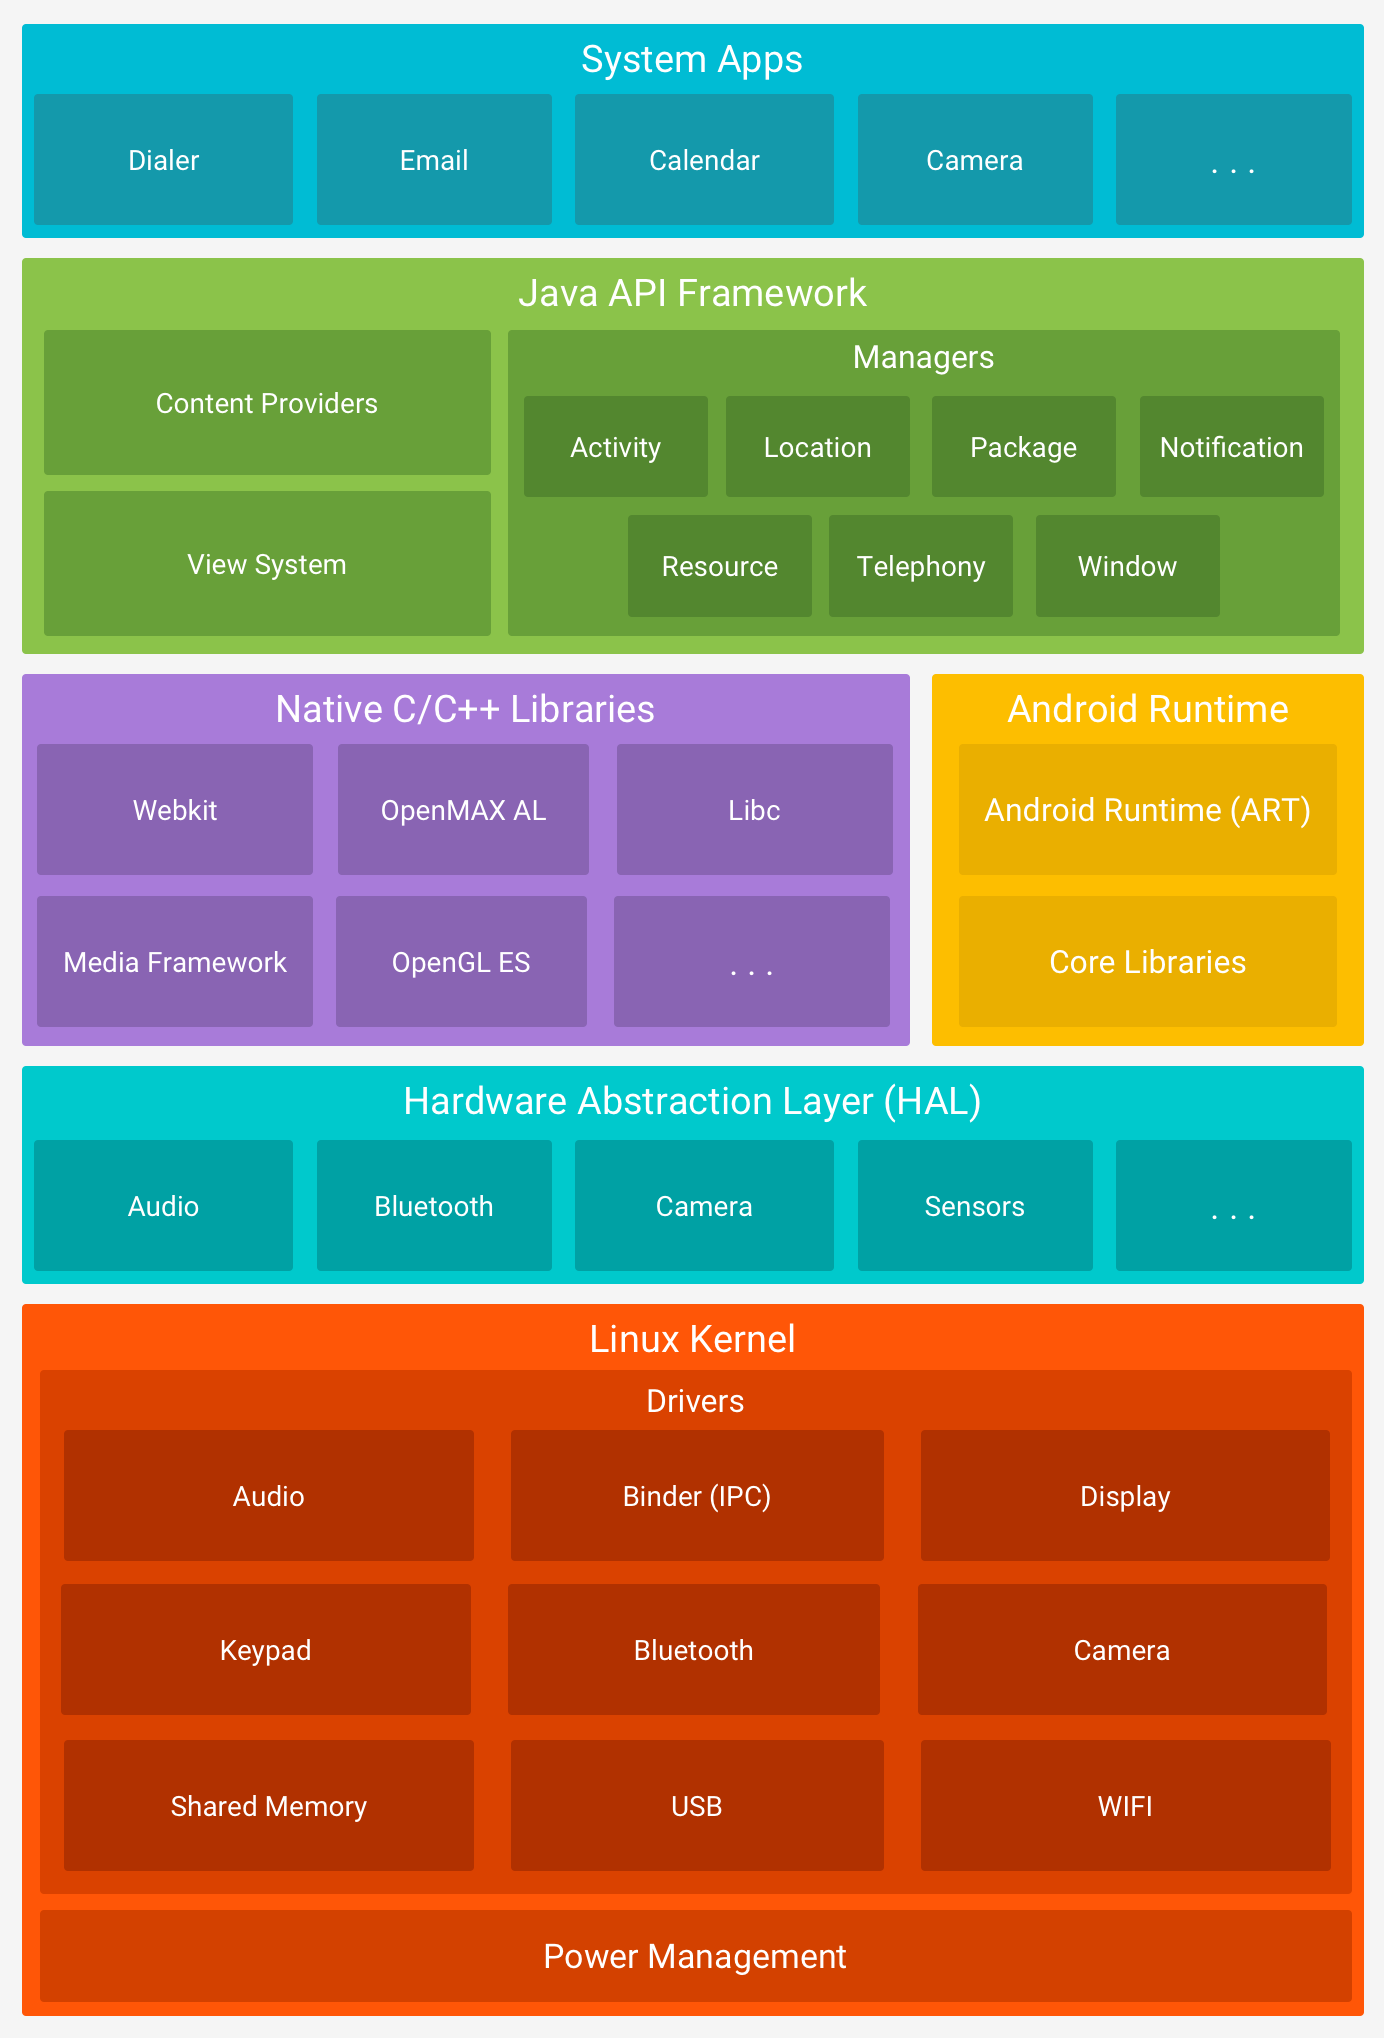
\includegraphics[scale=0.25]{imagenes/android-stack_2x.png}
	\caption{Pila de software de Android\cite{arquitecturaAndroid}\label{fig:arquitectura}}
\end{figure}

\subsection{Distribución de Android}
La distribución de Android viene a mostrarnos cual es el número de dispositivos que usan cada una de las versiones de Android. De hecho, el gran problema que aún presenta este sistema operativo es que pocos son los sistemas actualizados a la última versión disponible si los comparamos con el total, resaltando aún más al fijarnos en las estadísticas de iOS, el sistema de Apple, cuyos usuarios adoptan rápidamente la versión más reciente al poco tiempo de ser publicada. 

Gran parte de la culpa reside en el amplísimo número de marcas privadas que fabrican teléfonos con Android, cada una de las cuales con su propio hardware y su idea de cómo y cuando debería actualizar sus dispositivos. Esto acaba produciendo que muchas marcas sólo se preocupen de sus móviles más caros, y durante poco tiempo, creando un gran banco de usuarios con versiones de software desactualizadas, fallos de seguridad y sin las últimas novedades. 

Las estadísticas de distribución más recientes hasta el momento fueron publicadas en mayo de 2019, y son las siguientes:
\begin{figure}[H]
	\centering
	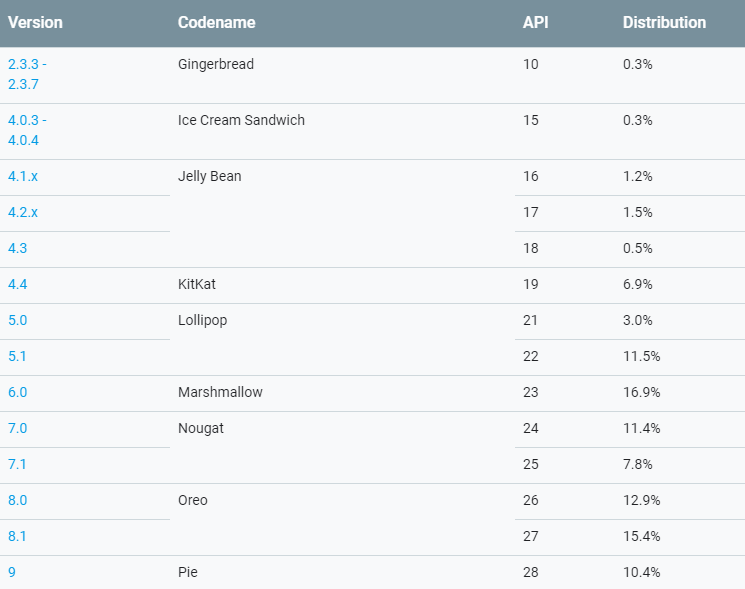
\includegraphics[scale=0.65]{imagenes/distribucion.png}
	\caption{Distribución de las versiones Android\cite{dashboards}\label{fig:distribucion}}
\end{figure}


\section{Opciones actuales en el mercado}

Son múltiples las guías y manuales sobre el test SPPB que se pueden encontrar en internet, donde se explica de forma detallada cuales son los pasos a tomar en cada prueba, los tiempos y los puntos. 

Sin embargo, no pasa igual si buscamos entre las aplicaciones de Google Play el término "SPPB". A pesar de ser el sistema operativo más usado del mundo, sólo dos de los resultados de la búsqueda están de algún modo relacionados con la valoración de fragilidad en ancianos, como se puede observar en la figura \ref{fig:google_play}. De ellas, no comentaremos la aplicación denominada ``Valoración de la Fragilidad''\cite{BlueBliss} puesto que en la práctica no posee ninguna opción para realizar el test SPPB.

\begin{figure}[H]
	\centering
	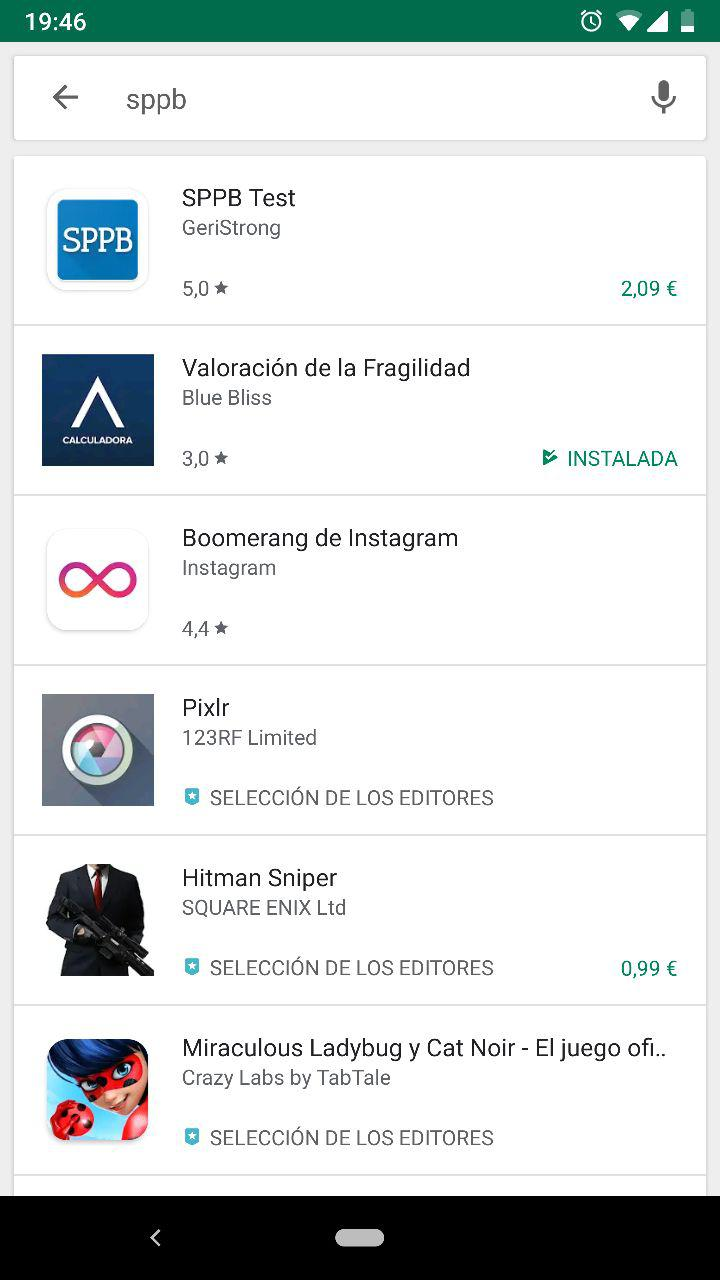
\includegraphics[scale=0.35]{imagenes/googlePlay_resultado.jpg}
	\caption{Resultados al buscar SPPB en la Google Play\label{fig:google_play}}
\end{figure}

La primera aplicación, de nombre ``SPPB Test''\cite{GeriStrong}, está enteramente dedicada a la realización y ejecución del test de Guralnik. Sin embargo, una primera pega que encontramos es su no gratuidad, que podría convertirse en un impedimento si pretendiésemos su uso entre la población anciana. A esto hay que sumarle que no es un proyecto de código abierto, con lo que no cabe la posibilidad de presentar mejoras ajenas a las que introduzca el propio creador.

\begin{figure}[H]
	\centering
	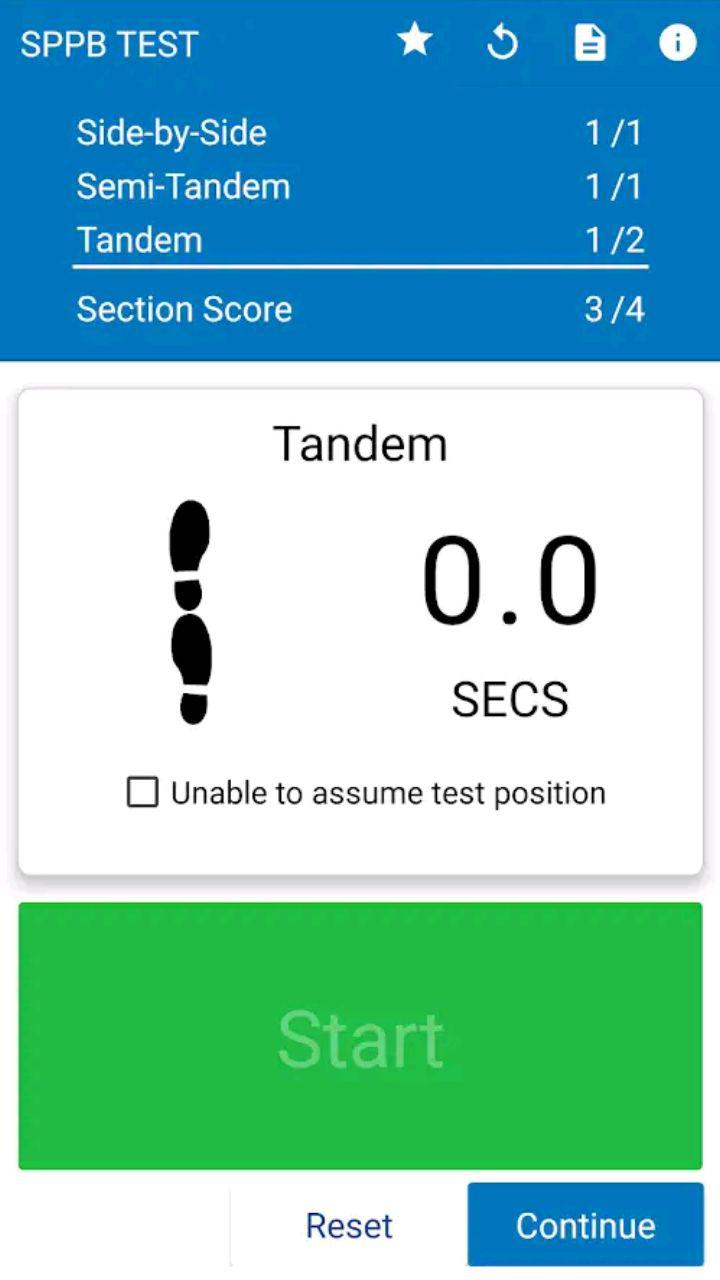
\includegraphics[scale=0.35]{imagenes/sppb_geristrong.jpg}
	\caption{Aplicación SPPB Test de GeriStrong\cite{GeriStrong}\label{fig:geriStrong}}
\end{figure}

Por otra parte, la aplicación parece sencilla de usar y ahorra la necesidad de elementos como un cronómetro o calculadora. Su enfoque está dirigido hacia el uso por parte de un médico o profesional, que guíe al paciente a través de las diferentes pruebas y controle la aplicación en todo momento. Además, es esa persona la encargada de comprobar y validar los movimientos que realiza el paciente, determinando si no se han llevado a cabo correctamente.

\section{Propuesta}

La propuesta que nosotros presentamos es la de crear una aplicación abierta y de código libre, sin ningún coste de compra, que esté orientada tanto al uso autónomo por parte de los ancianos como a su uso vigilado por un profesional. Además será muy importante la \textbf{integración del acelerómetro} presente en los móviles, que deberá encargarse de comprobar y validar la ejecución correcta de cada prueba.

Para conseguirlo, algunos de los puntos más importantes serán:
\begin{enumerate}
  \item Explicación clara y concisa del funcionamiento de cada una de las pruebas, tanto de forma escrita como mediante instrucciones guiadas por voz.
  \item Uso del acelerómetro para comprobar si cada prueba se ejecuta de forma correcta.
  \item Diseño bonito y adaptado a las pautas ofrecidas por Android.
  \item Posibilidad de guardar los resultados de múltiples usuarios.
\end{enumerate}

\chapter{Planificación}
En está sección vamos a explicar y desglosar varios aspectos relativos a la organización y desarrollo del proyecto como pueden ser sus etapas, la metodología empleada, herramientas de productividad y herramientas de desarrollo.

\section{Metodología usada}
La metodología que hemos empleado para el desarrollo de la aplicación es una de las pertenecientes al grupo de las \textit{ágiles}, cuyo nombre es \textbf{``SCRUM''}. 

La principal característica de ``SCRUM'' es la división del proyecto en otros más pequeños, cada uno de los cuales con sus propias etapas de análisis, diseño, desarrollo, etc. Dentro de la etapa de desarrollo se producen los denominados ``sprints'', que consisten, a grandes rasgos, en realizar regularmente entregas de una parte del proyecto para ser evaluadas.

Algunas de las ventajas que podemos obtener gracias al uso de esta metodología son la flexibilidad, la falta de grandes errores arrastrados por un desarrollo largo y una mayor libertad e innovación propiciados por el continuo planteamiento del proyecto\cite{VanessaRosello}.

Aplicado al desarrollo de nuestra aplicación, esto se traduce en la división del software en diferentes partes, cada una de las cuales se prueba con distintos usuarios a medida que se va completando. De este modo, es posible comprobar rápidamente qué partes del proyecto son más problemáticas y cuáles ofrecen mejores resultados, así como obtener una opinión general de los usuarios que puede y debe ser utilizada para guiar y replantear a tiempo múltiples partes del mismo. 

\section{Organización del proyecto}

\subsection{Etapas del proyecto}
\begin{itemize}
  \item \textbf{1ª etapa:} Estudio del problema.
  \item \textbf{2ª etapa:} Aprendizaje en Android.
  \item \textbf{3ª etapa:} Análisis de requisitos.
  \item \textbf{4ª etapa:} Planificación del proyecto.
  \item \textbf{5ª etapa:} Diseño de software e interfaz.
  \item \textbf{6ª etapa:} Implementación.
  \item \textbf{7ª etapa:} Pruebas.
  \item \textbf{8ª etapa:} Documentación.
\end{itemize}

Entre las etapas listadas anteriormente, aquellas que van desde la tercera hasta la séptima (ambas inclusive), se repetirán para cada una de las partes en las que estará dividido el desarrollo de la aplicación, como dicta la metodología ágil ``SCRUM'' utilizada.

\subsection{Descripción y temporización de las etapas}
\begin{itemize}
    \item \textbf{Estudio del problema.}
        \begin{itemize}
            \item \textbf{Descripción:} En esta etapa se llevan a cabo las conversaciones con el tutor para determinar la naturaleza del proyecto, así como obtener una idea más amplia del resultado que se pretende alcanzar. Se establece una planificación temporal para el resto de etapas.
            \item \textbf{Tiempo:} 3-4 horas.
        \end{itemize}
    \item \textbf{Aprendizaje en Android.}
        \begin{itemize}
            \item \textbf{Descripción:} Se realiza un proceso de auto-aprendizaje para la creación de aplicaciones para Android mediante la lectura de libros, guías, vídeos oficiales y documentación de la plataforma.
            \item \textbf{Tiempo:} 50 horas.
        \end{itemize}
    \item \textbf{Análisis de requisitos.}
        \begin{itemize}
            \item \textbf{Descripción:} Se realiza un estudio de las necesidades del usuario para determinar los requisitos del proyecto\cite{analisis_requisitos}. Se deciden las funciones que debe poseer el resultado final.
            \item \textbf{Tiempo:} 4-5 horas.
        \end{itemize}
    \item \textbf{Planificación del proyecto.}
        \begin{itemize}
            \item \textbf{Descripción:} Se divide el proyecto en distintas partes y se establece el orden de desarrollo.
            \item \textbf{Tiempo:} 1-2 horas. 
        \end{itemize}
    \item \textbf{Diseño de software e interfaz.}
        \begin{itemize}
            \item \textbf{Descripción:} Se realiza un boceto a mano alzada de la interfaz. Se lleva a cabo el diseño software de las distintas partes del proyecto.
            \item \textbf{Tiempo:} 8-9 horas. 
        \end{itemize}
    \item \textbf{Implementación.}
        \begin{itemize}
            \item \textbf{Descripción:} Se lleva a cabo el proceso de programación de todas las partes diseñadas. También se crean las imágenes e iconos que se necesitan en la aplicación.
            \item \textbf{Tiempo:} 240 horas.
        \end{itemize}
    \item \textbf{Pruebas.}
        \begin{itemize}
            \item \textbf{Descripción:} Tanto durante el desarrollo como al finalizar cada una de las partes del proyecto, se efectúan pruebas de forma personal y en distintos usuarios.  
            \item \textbf{Tiempo:} 6-7 horas.
        \end{itemize}
    \item \textbf{Documentación.}
        \begin{itemize}
            \item \textbf{Descripción:} Se crea un informe sobre el proceso de desarrollo del proyecto y otros aspectos.
            \item \textbf{Tiempo:} 70 horas.
        \end{itemize}
\end{itemize}

\newpage

\section{Tecnologías empleadas}

\subsection{Java}
El lenguaje que hemos utilizado para realizar la aplicación ha sido Java. Se trata de un lenguaje de programación que fue desarrollado por Sun Microsystems en el año 1995, aunque posteriormente fue adquirido por Oracle. 

Su principal característica es que, desde sus inicios, se planteó con el objetivo de que el código que los desarrolladores programasen pudiera servir en cualquier equipo, independientemente del sistema operativo. Para ello se intentó que tuviese el mínimo número de dependencias de implementación posible. Además, el código tras ser compilado, es ejecutado por una máquina virtual cuyo nombre es JVM, máquina que sí está adaptada y entiende el lenguaje del sistema operativo en cuestión, permitiendo así esa interoperabilidad y transversalidad.

En la actualidad se ha convertido en uno de los lenguajes de programación más populares y utilizados. Otras de sus características más importantes son la orientación a objetos y un recolector de basura que se encarga de eliminar todas las variables y objetos que ya no son referenciados por ningún elemento, lo que ayuda a evitar la mayoría de fugas de memoria\cite{java_wikipedia}.

\subsection{Android Studio}
La primera herramienta sobre la que hablaremos no podía ser otra que Android Studio, el instrumento por excelencia para crear aplicaciones para Android.

Android Studio es un entorno de desarrollo integrado (IDE por sus siglas en inglés) oficial, creado por la propia Google con el objetivo de sustituir a Eclipse, que era el editor usado anteriormente. Está basado en IntelliJ IDEA, aunque incorpora muchas acciones específicas muy útiles para la creación y desarrollo de apps. Fue anunciado en la Google I/O de 2013, pero su primera versión estable para todos los usuarios no estuvo disponible hasta diciembre de 2014\cite{android_developers, androidstudio_wikipedia}.

\begin{figure}[H]
	\centering
	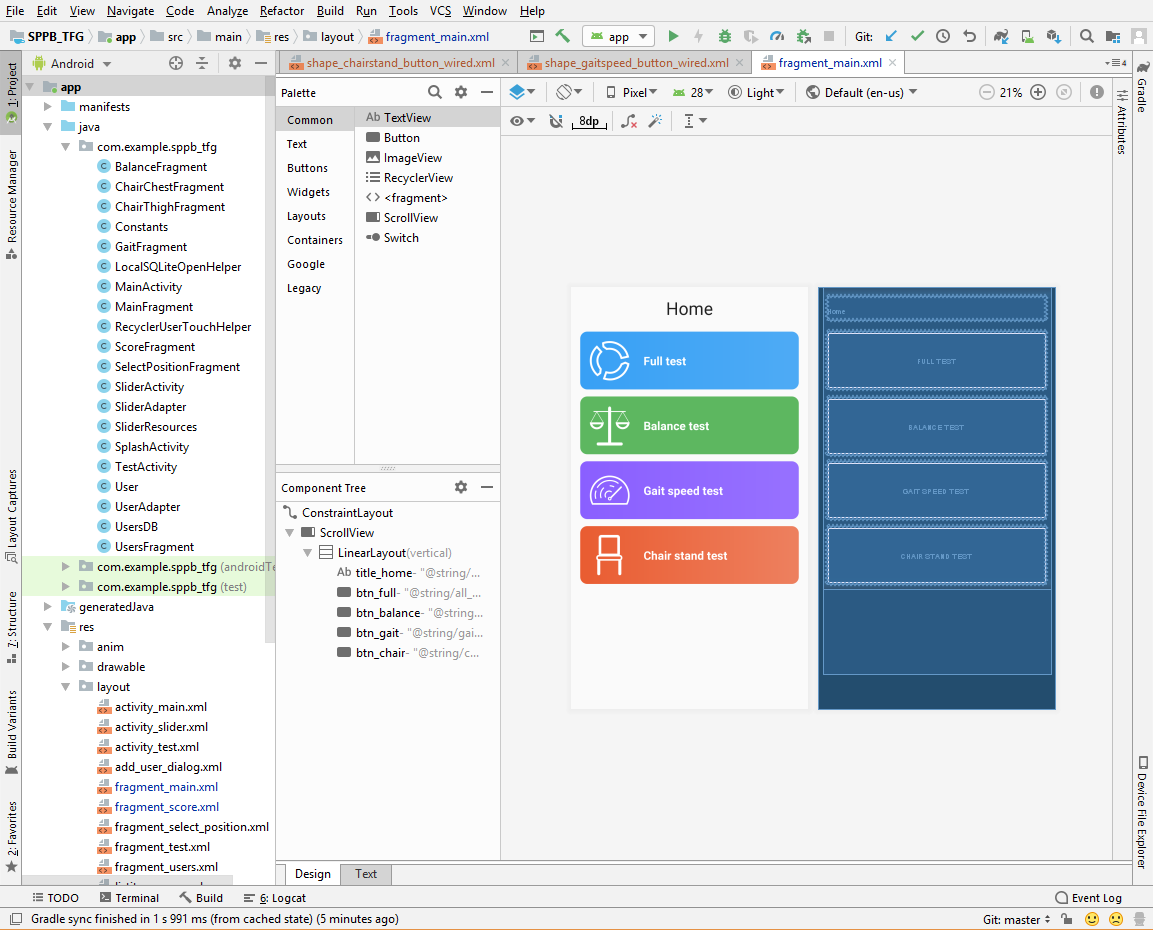
\includegraphics[scale=0.41]{imagenes/android_studio.png}
	\caption{Captura de pantalla de Android Studio\label{fig:android_studio}}
\end{figure}

Puede ser utilizado de forma completamente gratuita en las siguientes plataformas: Microsoft Windows, MacOS y GNU/Linux. Algunas de las principales características con las que cuenta son:
\begin{itemize}
    \item Emulador rápido con distintas funciones.
    \item Herramientas Lint, con la que es posible detectar problemas tales como bajo rendimiento, usabilidad, compatibilidad de versión, etc.
    \item Compatibilidad con C++ y NDK a parte de Java y Kotlin.
    \item Un sistema de compilación Gradle.
    \item Plantillas para los diseños más comunes.
    \item Renderizado en tiempo real.
\end{itemize}

\subsection{Github}
Otra de las herramientas más importantes del proceso ha sido Github. Github es una plataforma de desarrollo colaborativo, especialmente diseñado para alojar proyectos y permitir un control de versiones Git. Cuenta con muchas opciones como la de recuperar cualquier versión pasada del proyecto, indicar qué partes faltan por hacer, cuales están en progreso y cuales han acabado. También es posible comprobar qué usuarios han contribuido al desarrollo de un repositorio\cite{github_wikipedia}.

La principal utilidad que hemos dado a Github en este proyecto ha sido la de crear y mantener una copia de seguridad del código en cada momento, además de facilitar la compartición del mismo con los tutores y mostrarlo de forma pública para quien quiera usarlo, favoreciendo así el desarrollo colaborativo y la filosofía open source.

\subsection{Trello}
Trello es una plataforma online de productividad, enfocada en la gestión de proyectos. Imita a un tablero en donde se colocan notas dentro de diferentes categorías, las cuales pueden ser \textit{Por hacer}, \textit{En proceso} y \textit{Hecho}, entre otras. Además permite y facilita la creación de citas y avisos o el trabajo en equipo\cite{trello}.

\begin{figure}[H]
	\centering
	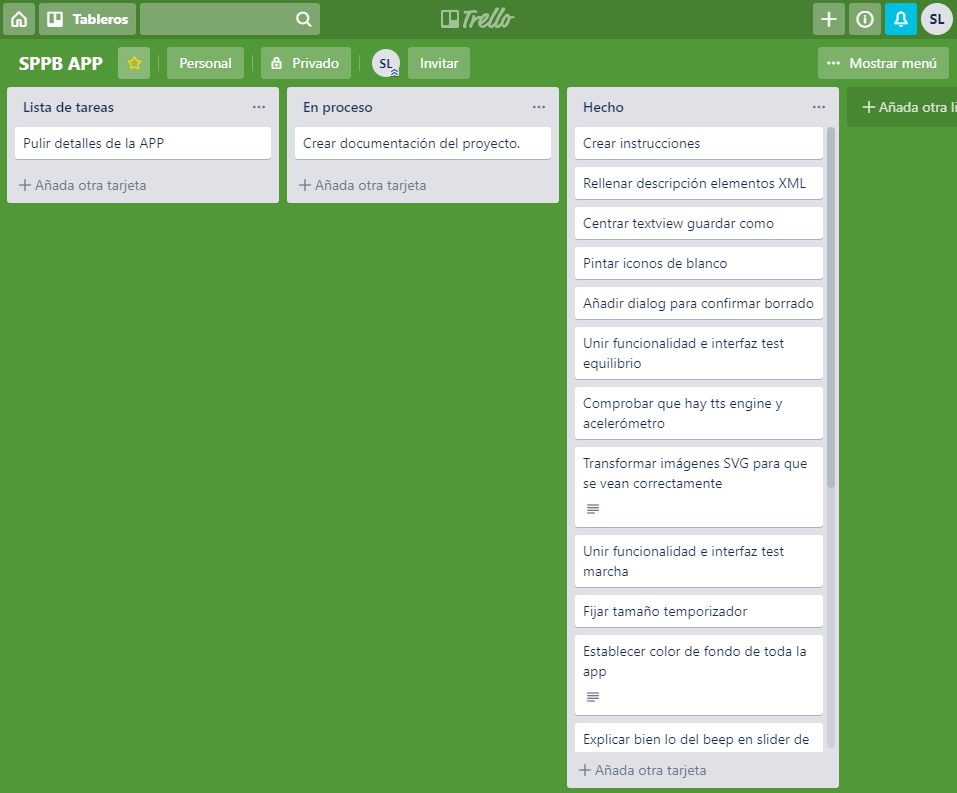
\includegraphics[scale=0.42]{imagenes/trello.png}
	\caption{Captura de pantalla de Trello.com\label{fig:trello}}
\end{figure}

Trello puede ser sustituido por la opción Issues que ofrece Github, puesto que su funcionamiento y cometido son muy similares. No obstante, debido a la gran facilidad de uso, nos hemos decantado por Trello en esta ocasión.

\chapter{Análisis}

En esta sección vamos a detallar toda la especificación que hay que realizar antes de comenzar a trabajar en cualquier proyecto software. Para ello, detallaremos los actores que participan, los requisitos funcionales, no funcionales y de información, entre otros aspectos.

\section{Descripción de los actores}

Debido a que la aplicación está orientada al uso local y exclusivo en el teléfono en el que sea instalada y que no hay necesidad de gestionarla de forma externa, habrá solo dos actores, uno principal al que llamaremos \textbf{usuario}, y un segundo actor, el \textbf{administrador}.

El \textbf{usuario} será la persona que se descargue la aplicación con el objetivo de realizar (él mismo o una tercera persona) el test SPPB. En principio, puesto que se buscará diseñar la aplicación para que sea lo más simple y explicativa posible, el usuario no debería necesitar de ninguna experiencia previa. 

El \textbf{administrador} se encargará únicamente de detectar, analizar y corregir errores que se puedan ir apareciendo en la aplicación, así como actualizarla regularmente con nuevas opciones y cambios que la mejoren.

\section{Análisis de requisitos}

Podemos encontrar tres tipos de requisitos, los \textbf{requisitos funcionales (RF)} que trazarán la interacción producida entre el sistema y el entorno, los \textbf{requisitos no funcionales (RNF)} que describirán características de la aplicación que no tienen relación con el comportamiento de la misma y \textbf{requisitos de información (RI)}, aquellos relacionados con la gestión y almacenamiento de información en el sistema.

\subsection{Requisitos funcionales}

\begin{itemize}
    \item \textbf{RF 1: Registro/creación de usuario.}
    \begin{itemize}
        \item El sistema permitirá al usuario escribir un nombre identificativo.
        \item El sistema creará la entrada correspondiente en la base de datos y lo almacenará.
        \item Se marcará el usuario recién creado como seleccionado.
    \end{itemize}
    
    \item \textbf{RF 2: Eliminación de usuario.} 
    \begin{itemize}
        \item Se podrá elegir un usuario a borrar mediante gesto de arrastre hacia la izquierda.
        \item El sistema comprobará la existencia del usuario a borrar.
        \item El sistema lo buscará y eliminará de la base de datos.
        \item En caso de que el usuario estuviera seleccionado para guardar resultados de test, el sistema lo deseleccionará antes del borrado.
    \end{itemize}
    
    \item \textbf{RF 3: Visualización de usuarios.} 
    \begin{itemize}
        \item El sistema mostrará una lista con todos los usuarios creados.
        \item Se mostrará información básica de cada uno de los usuarios de la lista (nombre y puntuación).
    \end{itemize}
    
    \item \textbf{RF 4: Selección/deselección de usuario.} 
    \begin{itemize}
        \item Se podrá seleccionar alguno de los usuarios guardados mediante una pulsación larga.
        \item El sistema mostrará y almacenará qué usuario está seleccionado desde ese momento en adelante.
        \item El usuario que se muestre como seleccionado almacenará los resultados de los futuros tests realizados previa confirmación.
        \item Se podrá deseleccionar un usuario previamente seleccionado mediante una pulsación larga.
    \end{itemize}
    
    \item \textbf{RF 5: Pantalla principal.} 
    \begin{itemize}
        \item Contará con cuatro botones, tres de ellos permitirán elegir una de las pruebas SPPB, el cuarto permitirá realizar las tres pruebas seguidas.
        \item Al pulsar uno de los botones, se abrirá una nueva actividad que permitirá realizar la acción deseada.
    \end{itemize}
    
    \item \textbf{RF 6: Instrucciones escritas.} 
    \begin{itemize}
        \item Si es la primera vez que el usuario abre un determinado test, se mostrará de forma automática una actividad con instrucciones escritas y visuales para su realización.
        \item Existirá un botón que permita volver a abrir las instrucciones cuando el usuario desee.
        \item Las instrucciones podrán cerrarse en cualquier momento.
        \item Las instrucciones mostradas serán distintas según el test desde el que se abran.
    \end{itemize}
    
    \item \textbf{RF 7: Instrucciones sonoras.} 
    \begin{itemize}
        \item Tras pulsar el botón de inicio (Play), se dictarán instrucciones de voz para guiar al usuario a través de la prueba.
        \item Las instrucciones de voz serán diferentes según el test seleccionado.
    \end{itemize}
    
    \item \textbf{RF 8: Silenciar instrucciones sonoras.} 
    \begin{itemize}
        \item Habrá un botón que permita silenciar las instrucciones sonoras al pulsarlo.
        \item Las instrucciones sonoras podrán volver a ser activadas tras pulsar el botón de nuevo.
    \end{itemize}
    
    \item \textbf{RF 9: Incapacidad para realizar la prueba.} 
    \begin{itemize}
        \item Habrá un botón que permita marcar la prueba como incapaz de realizarse.
        \item El sistema llevará automáticamente al usuario a la siguiente prueba (si procede) tras pulsar el botón.
    \end{itemize}
    
    \item \textbf{RF 10: Implementación pruebas SPPB.} 
    \begin{itemize}
        \item Deberán poder ejecutarse todas las pruebas que componen el test SPPB.
        \item Cada una de las pruebas debe realizarse conforme su diseño clínico.
    \end{itemize}
    
    \item \textbf{RF 11: Ejecución de la prueba.} 
    \begin{itemize}
        \item Cada prueba contará con distintos pasos por los que el sistema hará avanzar al usuario automáticamente.
        \item El usuario podrá tocar cualquier parte de la pantalla para continuar con la prueba.
    \end{itemize}
    
    \item \textbf{RF 12: Información del estado de ejecución de la prueba.} 
    \begin{itemize}
        \item En cada prueba, habrá un indicador que mostrará con texto el tiempo transcurrido en segundos o las repeticiones realizadas.
        \item Al finalizar la prueba, se mostrará una vista previa de los puntos obtenidos en dicha prueba.
    \end{itemize}
    
    \item \textbf{RF 13: Cambio automático de imágenes.} 
    \begin{itemize}
        \item La prueba irá acompañada con una explicación visual del estado actual de la misma.
        \item La explicación visual mostrará automáticamente en qué posición de equilibrio se encuentra el usuario, si se ha movido, si está caminando o parado, y si está de pie o sentado.
    \end{itemize}
    
    \item \textbf{RF 14: Tratado de datos procedentes del sensor acelerómetro.} 
    \begin{itemize}
        \item Se obtendrán datos del acelerómetro presente en el teléfono durante la ejecución de cada test.
        \item Se validarán y compararán los datos para comprobar los movimientos del usuario.
        \item El sistema determinará la duración de los movimientos del usuario y establecerá una puntuación en función de la misma.
    \end{itemize}
    
    \item \textbf{RF 15: Pantalla con puntuación.} 
    \begin{itemize}
        \item Se mostrará la puntuación total obtenida.
        \item Se mostrará la puntuación individual de cada una de las pruebas realizadas.
        \item Se indicará el nivel de limitación del usuario en base al resultado alcanzado.
        \item De haber realizado la prueba de velocidad de marcha, se mostrará el cálculo de velocidad media a parte de la puntuación.
        \item De haber algún usuario seleccionado antes de comenzar los tests, se dará la posibilidad de guardar el resultado en dicho usuario.
    \end{itemize}
    
    \item \textbf{RF 16: Elegir posición del teléfono para test de silla.} 
    \begin{itemize}
        \item Se dará la posibilidad al usuario de elegir colocar el dispositivo en el pecho o en el muslo antes de realizar el test de levantarse de la silla.
        \item Los datos del acelerómetro se interpretarán de forma distinta según la elección del usuario.
    \end{itemize}
\end{itemize}

\newpage

\subsection{Requisitos no funcionales}

\begin{itemize}
    \item \textbf{RNF 1:} La aplicación funcionará correctamente en la mayoría de teléfonos con API Android igual o superior a 21.
    \item \textbf{RNF 2:} \label{RNF:2} El peso de la aplicación no debe ser superior a los 7MB para poder ser usada en teléfonos con pocos recursos.
    \item \textbf{RNF 3:} La navegación entre las distintas pestañas y actividades debe ser fluida y rápida.
    \item \textbf{RNF 4:} El diseño ha de ser sencillo e intuitivo, y seguir la doctrina Material Theming en la medida de lo posible.
    \item \textbf{RNF 5:} \label{RNF:5} Todas las imágenes e iconos utilizados deben ser libres de derechos de autor o ser creadas ad hoc por los desarrolladores de la aplicación con el propósito de usarse en ella.
    \item \textbf{RNF 6:} La lista de usuarios almacenados ha de organizarse por orden alfabético del nombre.
    \item \textbf{RNF 7:} La pantalla ha de mantenerse encendida de forma continua durante la ejecución de los tests, pero no una vez finalizan.
    \item \textbf{RNF 8:} Se debe evitar un gasto desproporcionado de la batería suprimiendo el uso del acelerómetro una vez fuera de la actividad de los tests.
    \item \textbf{RNF 9:} No se han de requerir permisos especiales para el uso de la primera versión de la aplicación.
    \item \textbf{RNF 10:} Se evitará el uso del sensor giroscopio para permitir que teléfonos de baja gama utilicen la aplicación.
\end{itemize}

\subsection{Requisitos de información}

\begin{itemize}
    \item \textbf{RI 1: Información de usuarios.}
    \begin{itemize}
        \item Información sobre el nombre elegido, resultados del test y fecha de realización.
        \item Información sobre el usuario seleccionado actualmente.
    \end{itemize}
    
    \item \textbf{RI 2: Información de estado de la aplicación.}
    \begin{itemize}
        \item Se guarda la pestaña abierta antes de poner en pausa la aplicación, para abrirla de nuevo al continuar.
    \end{itemize}
\end{itemize}

\newpage

\section{Análisis de las soluciones}

Debido a que la aplicación por el momento no necesitará de conexión a internet ni de uso de una base de datos externa, no será necesario estudiar varios aspectos como la elección de un servidor, de una estructura del mismo o la seguridad de la conexión.

\subsection{Bases de datos}

Es posible encontrar distintos gestores de de bases de datos para usar en una aplicación para android. Algunos de los más importantes son\cite{databases}: 

\begin{itemize}
    \item \textbf{SQLite:} Se trata de un motor de bases de datos muy liviano y de código abierto. Algunas de sus principales ventajas es que no requiere de un servidor, puede trabajar de forma local, es sencillo de utilizar y no necesita ninguna clase de personalización o configuración. Su mayor problema se presenta cuando lo que buscamos es trabajar con bases de datos grandes.
    
    \item \textbf{CouchDB:} En este caso sí nos encontramos ante un \textbf{gestor} de bases de datos, también de código abierto. Está principalmente orientado a dar soporte a aplicaciones web y usa la estructura clave/valor de JSON para almacenar la información en documentos. Una de sus principales ventajas es que da la posibilidad de hacer copias de seguridad de los datos de forma sencilla, lo que puede ser muy útil en móviles para mostrar información cuando no disponen de conexión. 
    
    \item \textbf{FireBird:} FireBird es también un administrador de bases de datos de código abierto que hace uso del lenguaje de consultas SQL. Alguna de sus características principales es la gran escalabilidad que presenta (pudiendo trabajar bien ante un gran crecimiento sin perder eficiencia), interoperabilidad, seguridad, o una arquitectura cliente/servidor mediante conexiones TCP/IP.
    
    \item \textbf{MySQL:} Uno de los sistemas de gestión de bases de datos relacionales más conocidos. Es multiusuario y multihilo, open source, permite la arquitectura cliente/servidor,  etc.
    
    \item \textbf{PostgreSQL:} Por último, PostgreSQL es un gestor de BBDD relacional que también usa la arquitectura de cliente/servidor. Una de sus mejores características es el uso de multiprocesos que, a diferencia de los multihilos, evita que un problema causado en uno de los procesos perjudique al resto. Algunas otras características son su alta concurrencia o el acceso mediante SSL para una mayor seguridad.
\end{itemize}

\section{Solución propuesta}

La solución propuesta finalmente será utilizar el motor de bases de datos SQLite. Entre las razones principales podemos destacar el hecho de que no necesita un servidor, lo cual se ajusta a nuestras necesidades de almacenar la información de forma local. Además, al ser liviano, contribuimos al requisito no funcional 2 (\ref{RNF:2}) de no superar los 7 MB. Por otra parte, el problema de no ser bueno trabajando con bases de datos grandes no afectará a este proyecto ya que las necesidades son muy pequeñas.

\section{Análisis de seguridad}

En el aspecto de la seguridad no hemos visto la necesidad de prestar atención especial a ningún elemento concreto, puesto que la aplicación no cuenta ni requiere de conexión a internet, no se envían datos a ningún servidor o servicio externo, no es necesario el acceso a otros directorios del teléfono y la información que almacena de forma local no es sensible.

\section{Protección de datos}

El correcto tratamiento de los datos generados por los usuarios mediante la utilización de la aplicación no es sólo de vital importancia en el marco del proyecto, sino de obligado cumplimiento si nos atenemos al \textbf{Reglamento General de Protección de Datos} (GDPR por sus siglas en inglés) de la Unión Europea.

Este reglamento tiene como objetivo otorgar un mayor control a los usuarios sobre sus datos personales, entre los que se encuentra cualquier información que permita identificar a una persona, como por ejemplo la dirección IP, información económica, cultural, de salud mental, etc\cite{gdpr_eu, gdpr_powerdata}. 

Como los datos en ningún momento son enviados fuera de la aplicación ni procesados por terceras personas, el desarrollador de la aplicación no es controlador ni procesador de la información. Esta característica tiene como resultado que el \textbf{reglamento GDPR no afecta a esta aplicación}\cite{gdpr_stackexchange}. Por otra parte, el registro se hace de forma anónima ya que contiene datos sensibles relacionados con la salud, a lo que se añade que el usuario siempre cuenta con poder absoluto, pudiendo eliminar todos los datos sin que dejen rastro si así lo desea.

\chapter{Diseño}

En esta sección describiremos el diseño de la aplicación, tanto en el aspecto de la estructura de navegación como en el artístico y de interfaz.

\section{Estructura de navegación}

La estructura de navegación que hemos creado para la aplicación es sencilla y no muy extensa, persiguiendo el objetivo de conseguir la mayor facilidad de uso posible. De este modo, se evita un entramado laberíntico que empeora la experiencia de usuario.

En la siguiente figura (\ref{fig:navegacion}) podemos observar distintos elementos. Por una parte, tenemos las cuatro actividades que conforman la aplicación y que se muestran a continuación. A su vez, dentro de casi todas ellas hay fragmentos con distinta funcionalidad e interfaz: 
\begin{itemize}
    \item \textbf{Actividad splash:} Su función es únicamente mostrar una imagen mientras se inicia la aplicación.
    
    \item \textbf{Actividad principal:} Su contenido se alterna entre tres fragmentos distintos. Por una parte, el fragmento de inicio, el cual muestra y permite acceder a las diferentes partes del test SPPB. Por otra, el fragmento de usuarios, que muestra una lista con todos los usuarios guardados y la posibilidad de crear nuevos o borrar existentes. Por último, el fragmento de puntuación (que también es usado en la actividad tests), el cual exhibe la puntuación desglosada del usuario seleccionado.
    
    \item \textbf{Actividad tests:} En ella se muestran los fragmentos de las tres partes del test SPPB, cada uno con su propia funcionalidad. Al finalizar una de las pruebas o todas ellas, también aparece el fragmento de puntuación.
    
    \item \textbf{Actividad instrucciones:} Esta actividad alberga un elemento que ofrece Android denominado ViewPager, el cual permite deslizar la pantalla entre distintas diapositivas de instrucciones.
\end{itemize}

\begin{figure}[H]
	\centering
	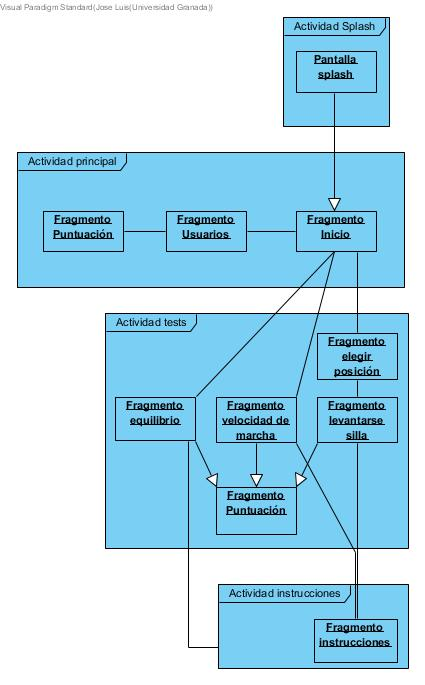
\includegraphics[scale=0.70]{imagenes/pantallas.jpg}
	\caption{Navegación entre pantallas\label{fig:navegacion}}
\end{figure}

\section{Diseño de la base de datos}

En este apartado describiremos el diseño propuesto para la base de datos. Como hemos apuntado anteriormente, las necesidades de almacenamiento serán muy básicas, siendo el objetivo guardar únicamente algunos datos producto de la realización de la prueba SPPB bajo un nombre o seudónimo elegido por el propio usuario.

\begin{figure}[H]
	\centering
	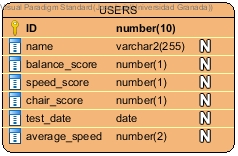
\includegraphics[scale=0.70]{imagenes/USERS.jpg}
	\caption{Diseño de la base de datos\label{fig:base_datos}}
\end{figure}

En la figura superior (\ref{fig:base_datos}) vemos un esquema UML de la base de datos. Podemos apreciar que sólo cuenta con una tabla que se usa tanto para almacenar el nombre como los resultados. El motivo radica en que la aplicación carece de la necesidad de administrar otros datos del usuario, los cuales podrían ser más sensibles y romper con el Reglamento General de Protección de Datos (GDPR). De este modo ahorramos tener que crear una tabla distinta destinada a guardar otros datos de identidad del usuario como podrían ser apellidos, edad o correo electrónico.

La única tabla, de nombre \textit{USERS}, cuenta con un total de 7 columnas. A parte de ID, usada para identificar mediante un número único a cada usuario, encontramos las siguientes:
\begin{itemize}
    \item \textbf{name:} De tipo texto, guarda el nombre o seudónimo introducido por el propio usuario para identificar la información de manera más sencilla.
    
    \item \textbf{balance\_score, speed\_score y chair\_score:} Todos de tipo numérico, ofrecen la posibilidad de registrar el resultado individual en las tres pruebas del test SPPB. Guardar dichos resultados individualmente garantiza la posibilidad de actualizar una prueba concreta a posteriori.
    
    \item \textbf{test\_date:} De tipo fecha, su objetivo es guardar en qué día se ha llevado a cabo el último test realizado. Aún no tiene uso, se guarda con vistas a añadir una funcionalidad futura.
    
    \item \textbf{average\_speed:} De tipo numérico, guarda la velocidad media calculada a raíz de la prueba de velocidad de marcha.
\end{itemize}

\section{Diseño de la interfaz}

El diseño de la interfaz ha sido una de las partes más importantes del desarrollo. Son muchas las razones que podemos dar e infinitos los artículos en internet que insisten encarecidamente en los beneficios de tomárselo en serio. Algunas razones listadas en el blog \textit{International Hispanic Community} \cite{design} son:
\begin{itemize}
    \item Hace que tu producto marque la diferencia.
    \item Da seriedad.
    \item Facilita la vida del usuario.
    \item Puede hacerte triunfar respecto a otras opciones.
\end{itemize}

Por todo ello, hemos preferido no mantener el diseño por defecto con el que cuentan los distintos elementos de la interfaz, dando un aspecto mucho más actual y con una mayor personalidad.

Es importante recalcar que tanto el diseño de la interfaz como el de las distintas imágenes se ha llevado a cabo sin ninguna noción de estilo, puesto que no es un ámbito que se imparta en el área de la programación. Por tanto, es muy probable que sean muchos los elementos que incumplan propiedades importantes dentro de la estructuración visual y gráfica que tendría que tener una interfaz, aunque se ha intentado conseguir un resultado profesional.


\subsection{Colores utilizados}

El color elegido como principal ha sido el azul (\#2196F3). Este se ha utilizado de forma recurrente en diferentes componentes como botones, textos y fondos. 

Por otra parte y con el objetivo de hacer más fácil de entender y recordar cada test mediante la asociación del mismo a un color, se ha decidido establecer una tonalidad diferente para cada una de las pruebas individuales. Finalmente, tras buscar combinaciones que resultasen agradables y fuesen suficientemente desiguales entre ellas, hemos optado por asignar una gama verde a la prueba de equilibrio (\#4CAF50), morada índigo a la prueba de velocidad de marcha (\#7C4DFF) y naranja al de levantarse de la silla (\#E64A19).

\subsection{Bocetos iniciales}

A la hora de determinar la apariencia y estructura gráfica de la aplicación, el primer paso no podía ser otro que un boceto hecho a mano alzada. Al realizarlo, obtenemos una primera impresión de cómo de bien o mal integrados estarían cada uno de los elementos. Además, al poder llevarse a cabo y modificarse de forma rápida y sencilla, es muy útil para mostrarlo a otras personas y obtener unas primeras opiniones que ayuden a modificar y mejorar el aspecto a lápiz, lo cual es mucho más efectivo que hacerlo más tarde sobre la interfaz real.

Puesto que la aplicación, al menos de momento, no tendrá demasiados apartados, ha sido relativamente fácil diseñar todas las pantallas que serán visibles al usuario. En total se trata de cuatro pantallas con diseños distintos. Habrá varios apartados que reutilicen los mismos diseños, como por ejemplo las pantallas visibles durante la ejecución de los tests. La estructura será la misma en todas ellas, pero cada una tendrá imágenes y color diferentes.

\begin{figure}[H]
	\centering
	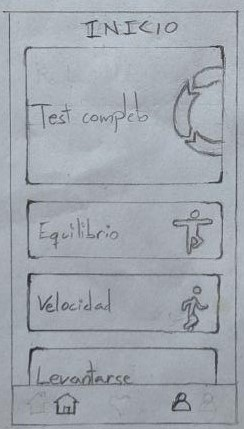
\includegraphics[scale=1]{imagenes/boceto_inicio.jpg}
	\caption{Boceto a lápiz de la pantalla de inicio\label{fig:boceto_inicio}}
\end{figure}

En la figura \ref{fig:boceto_inicio} podemos ver la idea inicial sobre cómo estructurar la \textbf{pantalla de inicio}. Cuenta con un título indicativo que reza \textit{INICIO}, útil para que el usuario sepa en qué pantalla se encuentra. Tras él, podemos ver cuatro botones, tres de ellos correspondientes a cada una de las pruebas que componen el test SPPB. Hay un cuarto botón, que en el boceto destaca más por su tamaño, el cual permite realizar el test completo (las tres pruebas que componen SPPB de forma seguida).

Por último se observa un menú inferior con únicamente dos opciones, la primera con un icono de una casa, para la pantalla Inicio, y la segunda con el icono de una persona, para la pantalla Usuarios.

\begin{figure}[H]
	\centering
	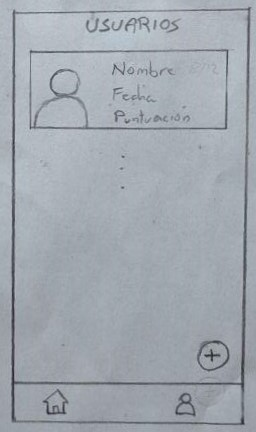
\includegraphics[scale=1]{imagenes/boceto_usuarios.jpg}
	\caption{Boceto a lápiz de la pantalla de usuarios\label{fig:boceto_usuarios}}
\end{figure}

Lo que puede observarse en la figura superior (\ref{fig:boceto_usuarios}) es la \textbf{pantalla de usuarios}. Como se puede comprobar, a parte del título hay una lista que pretende mostrar todos los usuarios guardados. Cada uno de los elementos muestra un nombre, una fecha de realización del test y una puntuación. No obstante, estos elementos se reducirán a uno sólo en la implementación, el del nombre, con el objetivo de que el texto pueda verse más grande y de que no se desfigure si las preferencias de tamaño de texto establecidas por el usuario son demasiado grandes. Así, facilitamos la accesibilidad al mejorar su optimización para personas con problemas de vista.

Por otra parte también se puede ver un icono de usuario, el cual también se modificará en la versión implementada, sustituyéndolo por un número con la puntuación obtenida. Este número adquirirá un color distinto dependiendo del rango de limitación en el que se encuentre, pasando desde rojo (en el peor caso), a naranja (limitación moderada), amarillo (limitación leve) y por último, verde (limitación mínima).

\begin{figure}[H]
	\centering
	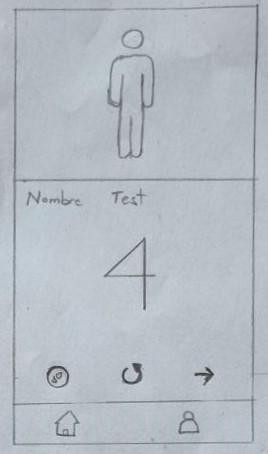
\includegraphics[scale=1]{imagenes/boceto_test.jpg}
	\caption{Boceto a lápiz de la pantalla de test\label{fig:boceto_test}}
\end{figure}

En esta imagen (figura \ref{fig:boceto_test}) se observa la que será la pantalla de ejecución del test. Se encuentra divida en aproximadamente dos mitades. La primera de ellas cuenta con una imagen en la que se mostrará un dibujo con la posición que se debe adoptar. Esta imagen se actualizará en caso de perder el equilibrio, de estar sentado o levantado, o de estar caminando o parado, añadiendo una mejor apariencia y un mayor dinamismo.

La otra mitad será la que albergue los controles y la información de ejecución. A parte del nombre del test actual, mostrará un botón de inicio (play) hasta el momento en el que sea pulsado. Posteriormente y a medida que se realiza el test, actualizará contadores como el cronómetro o el número de veces que se ha repetido el movimiento. Además, habrá botones para silenciar el sonido, para acceder a la información y para repetir la prueba o indicar incapacidad para realizarla.

\begin{figure}[H]
	\centering
	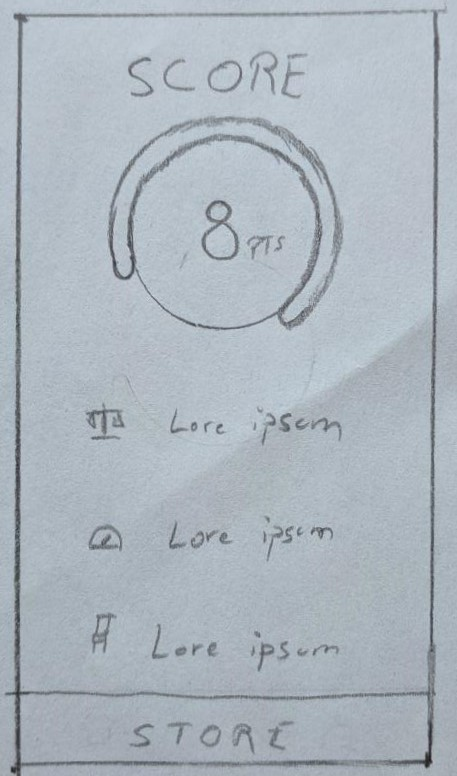
\includegraphics[scale=0.55]{imagenes/boceto_score.jpg}
	\caption{Boceto a lápiz de la pantalla de puntuación\label{fig:boceto_puntuacion}}
\end{figure}

Por último, en la figura \ref{fig:boceto_puntuacion} vemos lo que es una primera aproximación a la pantalla de puntuación. Esta pantalla será mostrada cuando pulsamos en algún usuario de la lista de usuarios o al finalizar un test, como vimos en el esquema de navegación entre pantallas de la figura \ref{fig:navegacion}. 

En ella mostraremos un círculo con progresión que estará más o menos relleno según la cantidad de puntos obtenida (entre 0 y 12). Posteriormente, se mostrará de forma individual el número de puntos alcanzados en cada uno de los tests. En caso de haber realizado una única prueba, se ocultarán los nombres e iconos de las no realizadas. Por último, también se podrá ver un botón de \textit{guardar} (STORE), mostrado únicamente si había un usuario seleccionado.

Esta vista también sufrirá cambios en la implementación, entre ellos la eliminación del título, la incorporación de un nuevo campo en el que se muestre el cálculo de velocidad media de marcha, o la sustitución de los iconos por un rectángulo pequeño con el color de cada prueba y el nombre.

\subsection{Imágenes utilizadas}

Como se indicó en el requisito no funcional número cinco (\ref{RNF:5}), es importante no usar imágenes o iconos con derechos de autor. No obstante, si queremos conseguir una apariencia con un estilo cohesionado y uniforme, la tarea se complica enormemente si pretendemos utilizar únicamente imágenes conseguidas de internet. Por ejemplo, es poco probable encontrar iconos que representen las tres partes del test SPPB con un diseño similar, y más improbable se vuelve aún hallar recursos gráficos parecidos de una silueta humana en las posiciones que requiere el test (tándem, sentado, andando, pérdida del equilibrio, etc).

Ante este problema, se tomó la decisión de realizar de forma personal toda la iconografía y diseños. Para tal fin, se utilizó una herramienta de diseño vectorial. Las imágenes vectoriales tienen la característica de no estar formadas por conjuntos de píxeles sino por formas geométricas y fórmulas matemáticas, las cuales permiten que la imagen nunca pierda calidad independientemente del tamaño con el que se redimensione. La gran ventaja que obtenemos es que, a parte de tener un tamaño mucho menor que las imágenes convencionales, no hay que preocuparse de cómo de grande es la pantalla del dispositivo en el que se muestre, puesto que siempre se visualizará con la máxima calidad posible\cite{vectorial}.

\subsubsection{Logotipo}

\begin{figure}[H]
	\centering
	
\includegraphics[scale=0.5]{imagenes/icon_small.png}
	\caption{Logotipo de la aplicación\label{fig:logo}}
\end{figure}

Dicho esto, comencemos mostrando y comentando el logotipo que se puede ver en la anterior figura (\ref{fig:logo}). Es un logotipo que busca ser simple pero mostrar a la vez la esencia de la aplicación. Se ha elegido darle forma de corazón por la relación del test SPPB con la detección de fragilidad en ancianos (capítulo \ref{ch:descripcion}) y las implicaciones en la salud que esto tiene. Además, se ha coloreado con los tres pigmentos establecidos para cada una de las partes del test, de forma que se resuma el estilo de la aplicación desde incluso antes de acceder a ella.

\subsubsection{Figuras de ejemplo}

\begin{figure}[H]
	\centering
	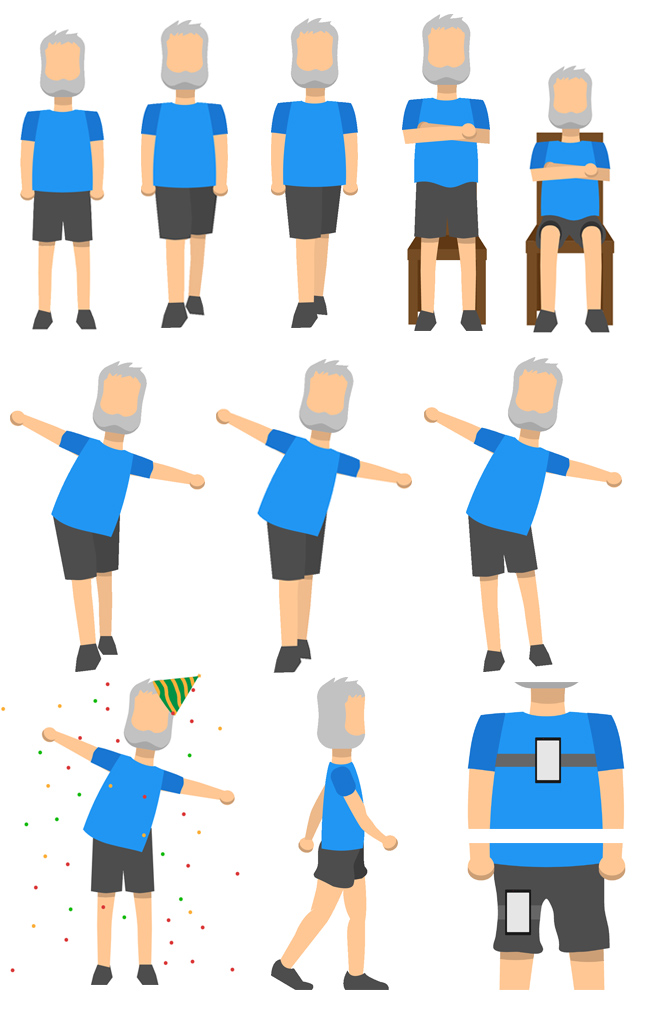
\includegraphics[scale=0.43]{imagenes/figuras_ejemplo.jpg}
	\caption{Todas las figuras de ejemplo para SPPB\label{fig:figuras_ejemplo}}
\end{figure}

En la imagen superior (\ref{fig:figuras_ejemplo}) podemos ver el personaje diseñado con el objetivo de mostrar la posición del test en cada momento, así como otra información relevante. Se trata de un diseño simple, sin apenas rasgos faciales ni de vestimenta para intentar convertirlo en lo más polivalente posible. 

Para diseñarlo nos hemos basado en un tutorial creado por Arumadigital \cite{Arumadigital} y en los personajes del programa de Mikel Izquierdo \cite{SPPB_clasificacion}, con el que hemos dado forma al primer personaje (arriba a la izquierda). Posteriormente, modificamos distintas partes y posturas hasta conseguir una variante del personaje que se adaptase a cada una de las posiciones necesarias.

\subsubsection{Iconos de los tests}

\begin{figure}[H]
	\centering
	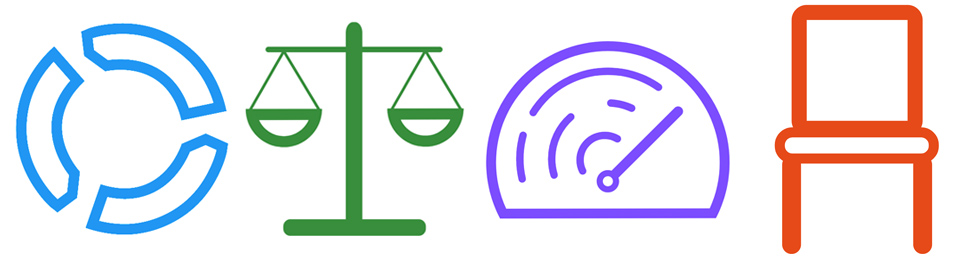
\includegraphics[scale=0.35]{imagenes/iconos.jpg}
	\caption{Todas los iconos de los tests SPPB\label{fig:todos_iconos}}
\end{figure}

En la figura \ref{fig:todos_iconos} vemos los cuatro iconos que aparecerán en cada uno de los botones que llevan a los distintos tests en la pantalla de inicio. Se ha intentado que tengan un estilo similar al estar formados por líneas y ningún relleno.

Aquí aparecen coloreados con su gama correspondiente, aunque en los botones de la pantalla de inicio serán blancos. Estos botones coloreados se usarán en otros elementos como los \textit{``Atajos''} de Android, que permiten acceder a una parte concreta de la aplicación desde fuera de la misma.

\newpage
\subsubsection{Imágenes varias}

\begin{figure}[H]
	\centering
	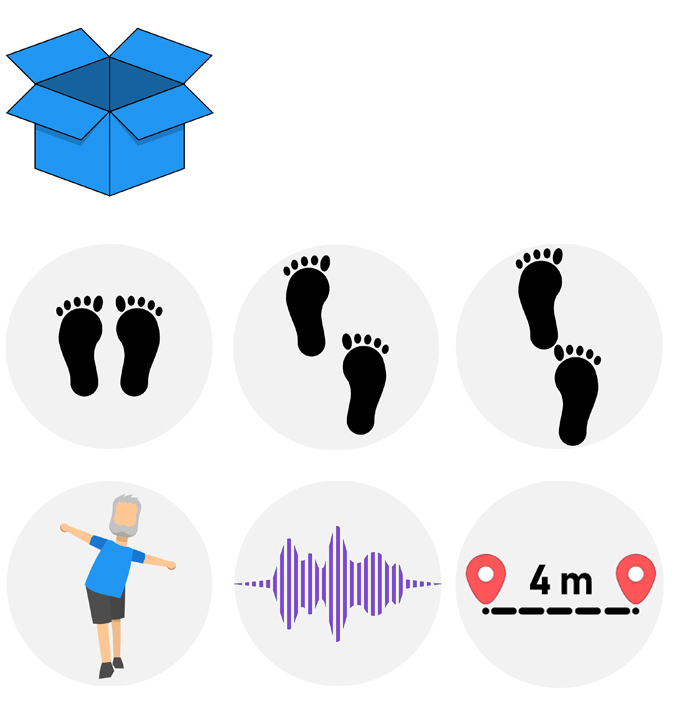
\includegraphics[scale=0.45]{imagenes/slides.jpg}
	\caption{Imágenes de instrucciones y miscelánea\label{fig:instrucciones}}
\end{figure}

Por último, en la figura \ref{fig:instrucciones} vemos siete dibujos más. El primero, la caja situada en primera fila, se utiliza para ilustrar gráficamente la pantalla de \textit{Usuarios} cuando no hay ningún usuario (valga la redundancia) almacenado. Al estar abierta y vacía, simboliza ausencia de elementos. Para realizarla nos basamos en un tutorial creado por The Simple Designers \cite{SimpleDesigners}.

En las dos siguientes filas se aprecian círculos que contienen distintas figuras de plantas del pie, sonido, distancia, etc. Han sido creadas con el objetivo de ser utilizadas en las diapositivas que pueden verse en la actividad de instrucciones. Hay varias imágenes de instrucciones que no aparecen aquí ya que para crearlas hemos reutilizado otras como las figuras de ejemplo \ref{fig:figuras_ejemplo}.

\subsection{Resultado final de la interfaz}

A continuación veremos el resultado final del diseño. Aquí sí podrán apreciarse la aplicación de colores y la integración de imágenes, cosa que en los bocetos a mano alzada no se conseguía. 

\begin{figure}[H]
	\centering
	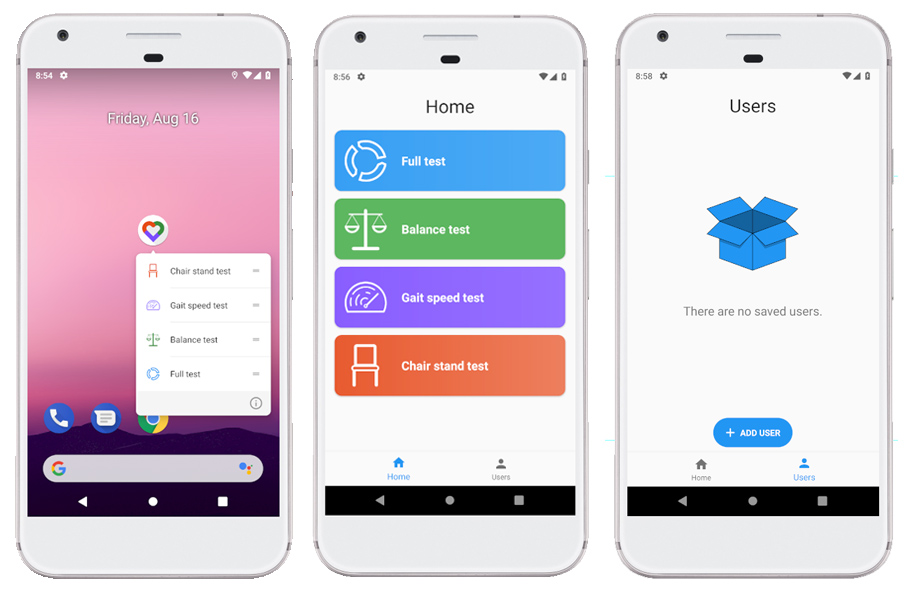
\includegraphics[scale=0.4]{imagenes/capturas1.jpg}
	\caption{Pantallas principales de la aplicación\label{fig:capturas1}}
\end{figure}

En la figura superior (\ref{fig:capturas1}) se observan tres pantallazos. En el primero de ellos aparece el acceso directo a la aplicación, que se muestra con el logotipo del corazón. Si nos fijamos, hay un menú desplegado que cuelga del icono de la app. Este menú cuenta con cuatro de los denominados \textit{atajos} de Android que mencionamos anteriormente y que permiten acceder a cualquiera de las tres pruebas de forma directa, o a la ejecución completa del test SPPB. Se trata de funcionalidades sin demasiada importancia pero que pueden ser útiles en un determinado momento.

En segundo lugar vemos la que finalmente es la \textbf{pantalla principal} de la aplicación. En ella hay cuatro botones con un ligero degradado como ya se adelantó en el boceto, aunque el tamaño y la forma de todos ellos no es igual que en la idea original.

Por último encontramos la \textbf{pantalla de usuarios}. Al no haber ningún usuario guardado, se muestra el dibujo por defecto de la caja vacía junto a un texto explicativo. También hay en esta pantalla un botón azul (el color principal de la aplicación) para añadir usuarios. Ese botón se oculta en caso de que haya una lista superior al tamaño de la pantalla y se realice un desplazamiento o \textit{scrolling} hacia abajo, para volver a mostrarse cuando se realiza hacia arriba.

\begin{figure}[H]
	\centering
	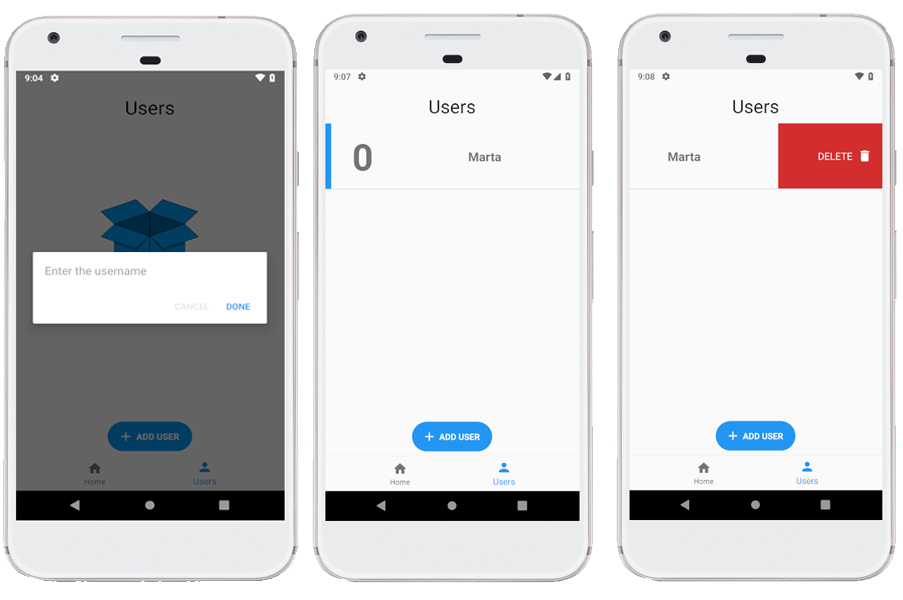
\includegraphics[scale=0.4]{imagenes/capturas_usuarios.jpg}
	\caption{Pantallas de usuarios\label{fig:capturas_usuarios}}
\end{figure}

En la figura \ref{fig:capturas_usuarios} se aprecian más comportamientos de la misma. Por una parte y en primer lugar, tenemos una captura (la situada en la izquierda) en la que se ve un cuadro de diálogo que se muestra al tocar el botón azul de añadir usuarios y que permite realizar lo propio.

En segundo lugar, una vez almacenado el primer usuario, se ve cómo desaparece la caja y texto explicativo por defecto y aparece una fila con un cero (la puntuación actual en los tests) y un nombre de usuario introducido anteriormente. Si nos fijamos, vemos además una línea vertical azul que aparece por defecto y que puede quitarse o volver a ponerse mediante una pulsación larga. Esta línea indica que el usuario se encuentra seleccionado, con lo que al realizar el test nos dará la opción de guardar la puntuación en este usuario.

En la última captura (la más a la derecha) se ve la posibilidad de borrar un determinado usuario mediante un gesto de arrastre. Si dicho gesto se lleva a término, aparecerá un cuadro de diálogo que nos pedirá confirmación antes de eliminarlo completamente, de forma que se eviten quitar algún usuario de forma inintencionada. Esto es importante ya que al almacenarse todos los datos de forma local únicamente, sería imposible recuperar esta información.

\begin{figure}[H]
	\centering
	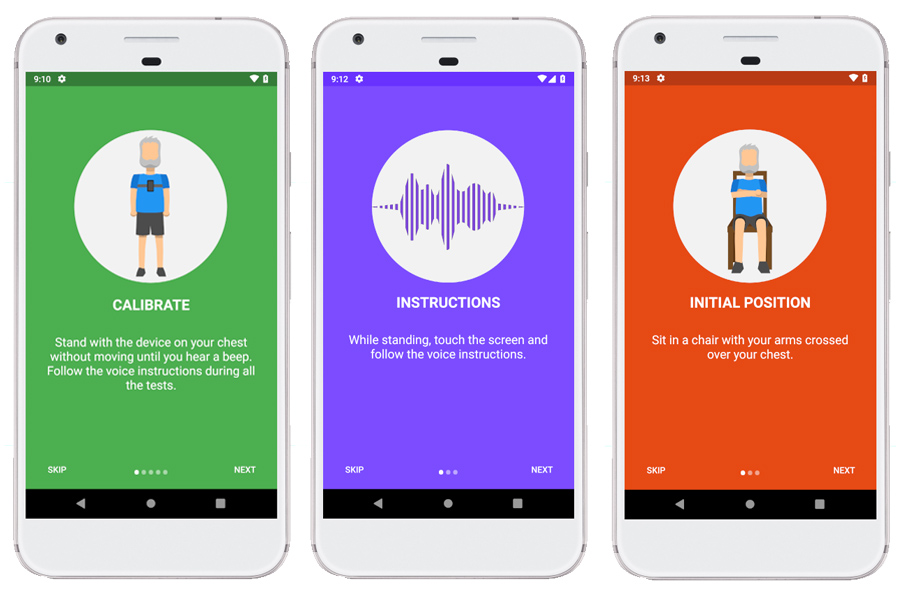
\includegraphics[scale=0.4]{imagenes/capturas_instrucciones.jpg}
	\caption{Pantallas de instrucciones\label{fig:capturas_instrucciones}}
\end{figure}

En este caso, en la figura \ref{fig:capturas_instrucciones} vemos un ejemplo de cómo son las pantallas de instrucciones de cada uno de los distintos tests.

La principal característica común y que a la misma vez sirve para diferenciarlos es el color de fondo. Las instrucciones de la primera captura pertenecerían pues al test de equilibrio, la de la segunda captura al de velocidad de marcha y las de la tercera, al test de levantarse y sentarse cinco veces en una silla. Además, todas ellas tienen un tono más oscuro de ese mismo color para la barra de estado (efecto que hay que programar y que en ningún caso viene por defecto). 

También vemos en todas una imagen, un título y una descripción. Es posible deslizar el dedo a izquierda o derecha para avanzar por las instrucciones. En la parte inferior se observan dos botones y unos puntos que sirven para indicar cuantas diapositivas quedan por ver y cuantas se han visto ya. Además, estos botones que hemos mencionado también permiten navegar entre ellas, moviéndonos de una en una a la siguiente o la anterior, finalizar cuando nos encontramos en la última diapositiva o saltarnos las instrucciones si lo deseamos cuando estamos en la primera.

La actividad de instrucciones aparece de forma automática si es la primera vez que se abre un determinado test tras descargar la aplicación. Posteriormente, pueden consultarse de nuevo todas las veces que haga falta pulsando el botón de información que aparece en las primeras capturas de la figura \ref{fig:capturas_test}.

\begin{figure}[H]
	\centering
	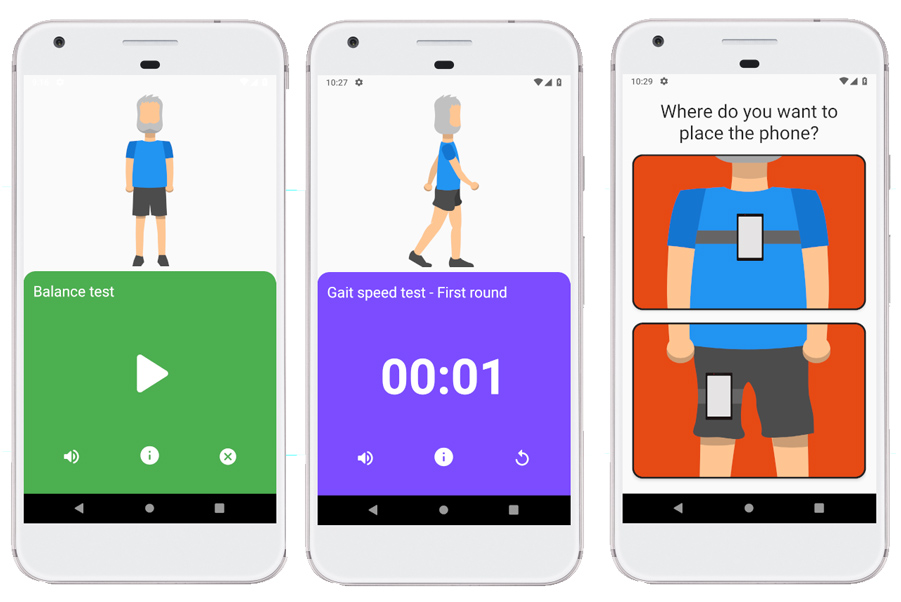
\includegraphics[scale=0.4]{imagenes/capturas_test.jpg}
	\caption{Pantallas de test\label{fig:capturas_test}}
\end{figure}

En la figura \ref{fig:capturas_test} vemos de nuevo tres capturas, correspondientes en este caso a la pantalla de realización de los tests.

Al igual que ocurría en las instrucciones, la mitad inferior que contiene los controles y la información del test establece el color de fondo según qué prueba se está realizando, pudiendo variar entre verde, morado índigo y naranja. La mitad superior alberga una imagen de ejemplo como ya diseñamos en los bocetos a mano alzada, imagen que cambia y se adapta según la parte del test en el que estemos. Por ejemplo, en la prueba de velocidad de marcha se observa como la figura se encuentra en posición de caminar, figura que cambia cuando el usuario deja de realizar el movimiento. 

En la mitad inferior vemos el título de la prueba (e información extra como la posición de los pies que toca en cada momento o la repetición actual del test de marcha), y cuatro controles. El primero es un botón de iniciar (play) que desaparece al clicarlo, y los otros tres son por este orden: silenciar las instrucciones, información y repetir la prueba/incapacidad para realizar la prueba.

En la tercera imagen se aprecia un diseño distinto. Esto se produce únicamente como paso previo al test de silla, el cual sí tiene un diseño similar al de las dos pruebas anteriores. Lo que se hace en esa pantalla es preguntar al usuario el lugar donde querrá colocar el dispositivo, pudiendo elegir entre el pecho y el muslo. Las razones por las que añadimos esta capacidad de elección se explicarán posteriormente y tienen que ver con la fiabilidad de medición del acelerómetro.

\begin{figure}[H]
	\centering
	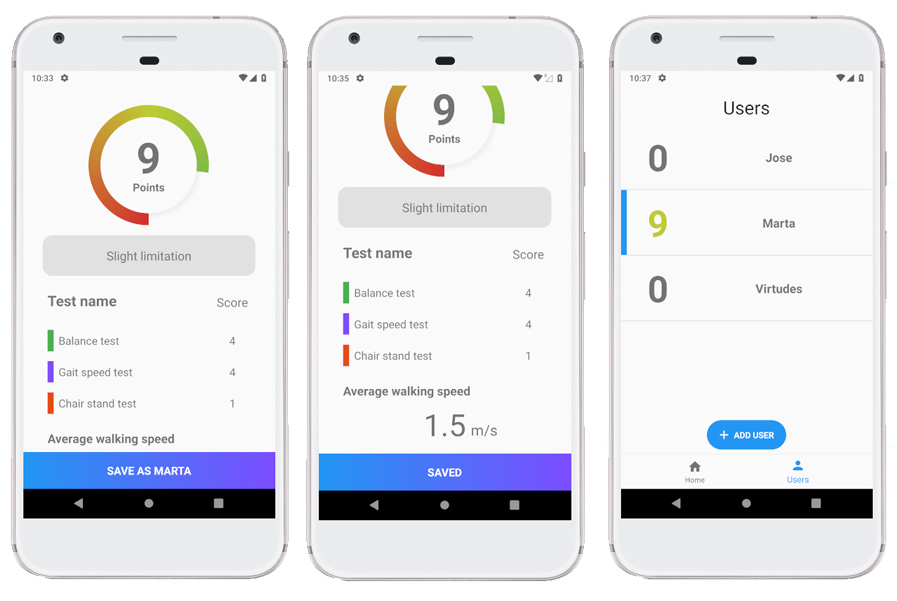
\includegraphics[scale=0.4]{imagenes/capturas_puntuacion.jpg}
	\caption{Pantallas de puntuación\label{fig:capturas_puntuacion}}
\end{figure}

En último lugar comentaremos la figura \ref{fig:capturas_puntuacion}. Es muy similar al diseño realizado en el boceto, salvo pequeños cambios. Esta pantalla aparece tras finalizar alguno de los tests, los tres test o al pulsar uno de los usuarios almacenados de la lista.

En primer lugar contiene un círculo en el que se muestra la puntuación total obtenida y la progresión que supone respecto al total alcanzable. Debajo hay un cuadro con una etiqueta que informa del grado de limitación al que equivale la puntuación conseguida, pudiendo variar desde \textit{limitación grave} en el peor de los casos a \textit{limitación mínima} en el mejor.

Si continuamos descendiendo, encontramos un desglose por pruebas de la puntuación de cada una. Más abajo, si desplazamos la pantalla, aparece la velocidad media de marcha, calculada a raíz de la prueba de velocidad de marcha. Este indicador puede ser muy útil en cuanto a significado clínico.

En último lugar encontramos un botón que aparece en caso de tener un usuario seleccionado antes de iniciar el test. Dicho botón nos ofrece la posibilidad de almacenar el resultado en tal usuario, de forma que la puntuación se mostrará actualizada en la lista, y se nos permitirá acceder en cualquier momento para consultar el desglose de la última ejecución del test.

\chapter{Implementación}

Esta sección estará dedicada a explicar aspectos tanto de la creación y desarrollo de los algoritmos de medición en las pruebas como del resto de elementos de la aplicación, señalando pequeños detalles que hayan podido generar problemas o que tengan alguna relevancia.

\section{Funcionamiento del acelerómetro}
\label{sec:acc}

Antes de proceder con el diseño e implementación de los algoritmos de medición para las pruebas del test SPPB, es importante comprender qué es el acelerómetro, qué mide y cómo funciona.

El acelerómetro es un pequeño sensor que incorporan la gran mayoría de los teléfonos vendidos hoy en día. Su cometido es medir \textbf{cambios en la velocidad de movimiento} del dispositivo que se produzcan en cualquiera de los tres ejes. Es decir, es bueno detectando \textbf{aceleración}.

\begin{figure}[H]
	\centering
	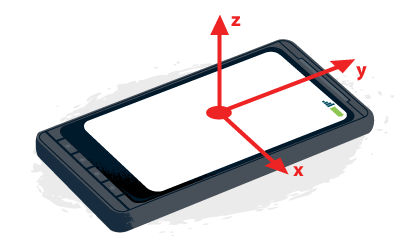
\includegraphics[scale=0.4]{imagenes/axes_mobile.png}
	\caption{Ejes del acelerómetro\label{fig:ejes_acc} \cite{PeteLepage}}
\end{figure}

Si tenemos en cuenta que la gravedad es una fuerza que se mide en unidades de aceleración \cite{gravedad}, podemos obtener también la \textbf{orientación y giros} del dispositivo gracias a la interpretación de la información recibida en cada eje. Por ejemplo si un teléfono móvil está sobre la mesa, recibirá una fuerza en su eje Z similar a la constante de gravedad que genera la tierra, y unos valores cercanos a cero en los ejes X e Y representados en la figura \ref{fig:ejes_acc}.

Por intentar buscar un equivalente, el acelerómetro obtiene datos parecidos a si nosotros tuviésemos los ojos vendados. Al ser movidos, podríamos detectar en qué dirección nos llevan y la orientación de nuestro cuerpo, pero no en qué lugar estamos ni la altitud.

\section{Test de levantarse de la silla}

Este fue probablemente el test más complejo de desarrollar. Como hemos mencionado anteriormente, no es posible detectar la posición ni la altura del dispositivo mediante el uso exclusivo del acelerómetro. Por ejemplo, si el usuario se encuentra de pie o sentado y no se mueve, siempre que el móvil esté sujeto a la zona requerida para este proyecto (el pecho, con orientación vertical) no habrá forma de inferir cual de las dos mencionadas posiciones es la vigente. La razón es que el eje Y marca el mismo valor de gravedad en ambas situaciones mientras que los ejes X y Z marcan cero. La única forma por tanto de determinar la posición actual del usuario sería medir los cambios de aceleración producidos en el proceso de levantarse o sentarse. 

\begin{figure}[H]
	\centering
	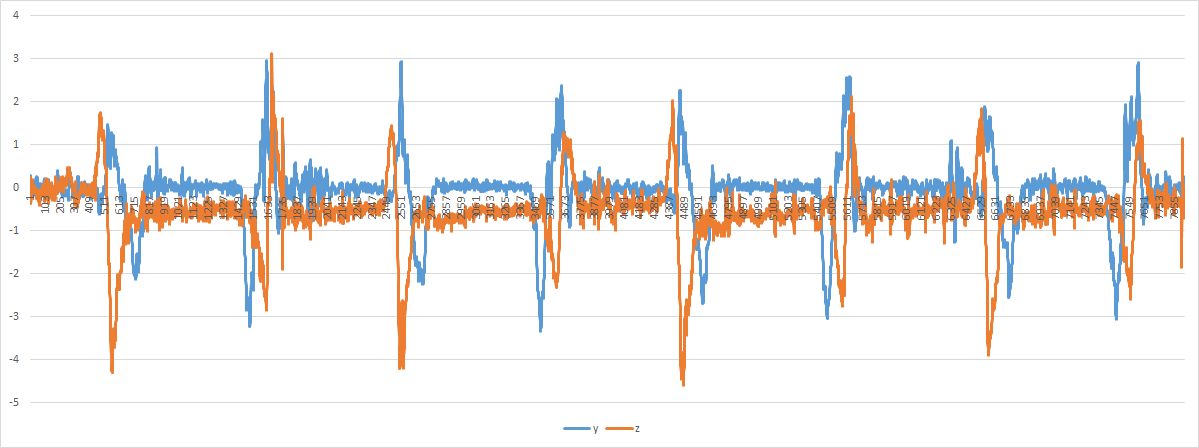
\includegraphics[scale=0.395]{imagenes/grafico_completo_silla_vacio.png}
	\caption{Datos del acelerómetro al levantarse y sentarse.\label{fig:acc_1}}
\end{figure}

Si nos fijamos en la imagen superior (figura \ref{fig:acc_1}) podemos apreciar una gráfica de datos obtenidos por el acelerómetro de un teléfono. La recolección de datos se ha llevado a cabo gracias a una aplicación llamada \textit{``Physics Toolbox Accelerometer''}\cite{Vieyra}. En la gráfica hemos representado solamente los ejes Y (azul) y Z (naranja) por ser los únicos que muestran cambios significativos en el desarrollo del test.

\begin{figure}[H]
	\centering
	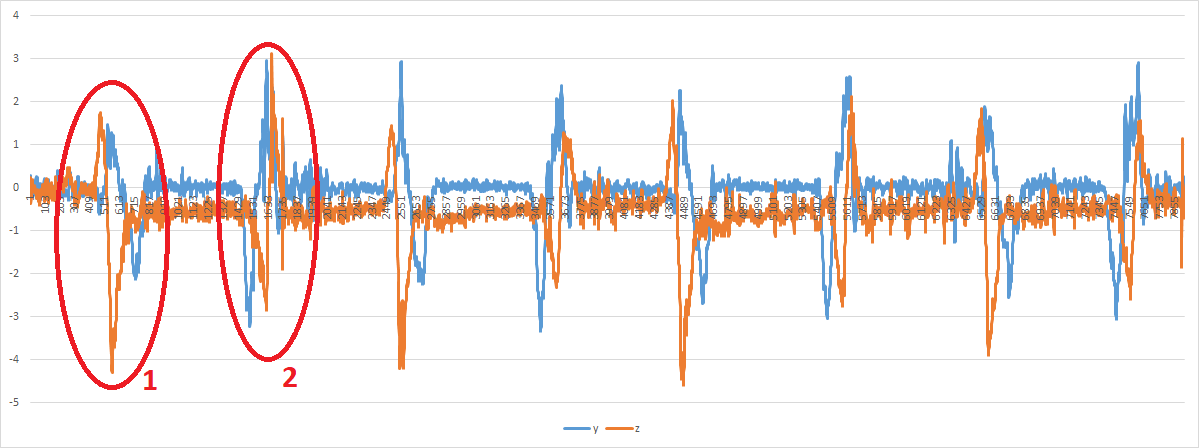
\includegraphics[scale=0.395]{imagenes/grafico_completo_silla.png}
	\caption{Datos del acelerómetro al levantarse y sentarse 2.\label{fig:acc_2}}
\end{figure}

La medición de la gráfica tuvo lugar comenzando desde una posición origen sentado, con lo que los cambios apreciables en la etiqueta 1 corresponden al proceso de levantarse, mientras que los de la etiqueta marcada con un 2 equivalen a sentarse de nuevo. Todas las fluctuaciones intermedias que tienen lugar son debidas en su gran mayoría a ruido en los datos.

Durante el resto de la gráfica, aunque no esté etiquetada, se repite el proceso de levantarse y sentarse hasta en tres ocasiones más. Si lo analizamos más a fondo, podemos encontrar un patrón en los datos de forma relativamente sencilla. Usaremos gráficas con ejes representados individualmente para analizarlos mejor.

\begin{figure}[H]
	\centering
	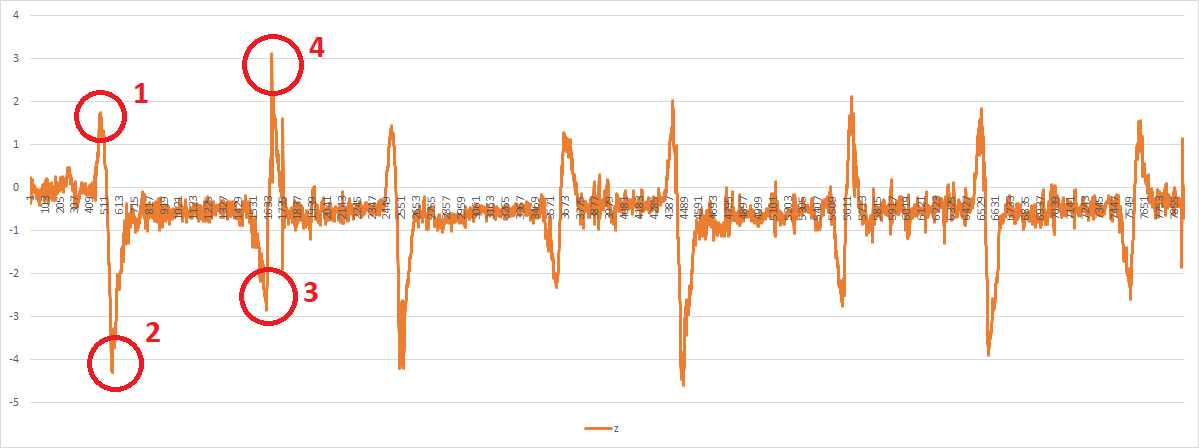
\includegraphics[scale=0.395]{imagenes/grafico_z_silla.png}
	\caption{Datos del acelerómetro al levantarse, eje Z.\label{fig:acc_3}}
\end{figure}

Al levantarnos desde una silla, todo nuestro tronco superior (y con él, el móvil) avanza hacia el frente. Este movimiento de avance, que corresponde al eje Z de nuestro dispositivo mientras lo tengamos sujeto al pecho, se aprecia en la etiqueta 1 de la figura \ref{fig:acc_3}. En ella se llega a alcanzar un pico de casi 2 m/$s^{2}$ de aceleración que al detenerse, provoca una aceleración inversa del dispositivo señalada en la etiqueta número 2.

Cuando procedemos a sentarnos, el tronco se desplaza hacia atrás, provocando un movimiento negativo en el eje Z. Esto encaja con la representación de la etiqueta 3, en la que se ve una aceleración negativa cercana a los -3 m/$s^{2}$, con su correspondiente aceleración inversa al detenerse (una vez sentados completamente) que figura en la etiqueta 4.

Si nos fijamos, los cambios registrados al levantarse y sentarse siguen el mismo patrón pero con signo opuesto. Además, este patrón se repite una y otra vez durante el resto de la gráfica: siempre que hay una aceleración positiva y justo después una negativa, se habrá producido un movimiento de avance en el eje Z necesario para incorporarse, y siempre que haya una aceleración negativa inmediatamente seguida por una positiva, será el movimiento de retroceso (típico al sentarse) el que se haya llevado a cabo.

\begin{figure}[H]
	\centering
	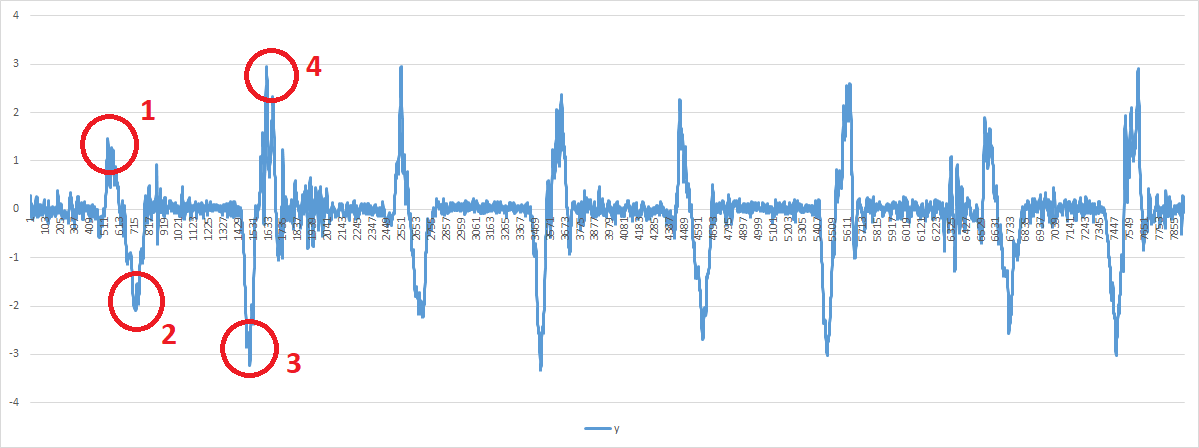
\includegraphics[scale=0.395]{imagenes/grafico_y_silla.png}
	\caption{Datos del acelerómetro al levantarse, eje Y.\label{fig:acc_4}}
\end{figure}

Los datos del eje Y que aparecen en la figura \ref{fig:acc_4} son casi idénticos a los registrados en el eje Z, salvo por un pequeño desfase entre ambos debido principalmente a que solemos inclinarnos hacia delante antes de levantarnos, y empezamos a sentarnos antes de desplazarnos hacia atrás.

Por lo demás, el comportamiento es el mismo. Al levantarnos, nuestro tronco superior sube y el acelerómetro detecta una aceleración positiva (etiqueta 1). Al detener la subida, se vuelve a obtener aceleración inversa como se ve en la etiqueta 2. El procedimiento se vuelve a repetir con valores inversos al sentarnos.

Aunque en esta gráfica parece muy fácil determinar cuándo el usuario se encuentra de pie y cuándo se ha sentado, la tarea se complica bastante en los siguientes casos.

\newpage

\begin{figure}[H]
	\centering
	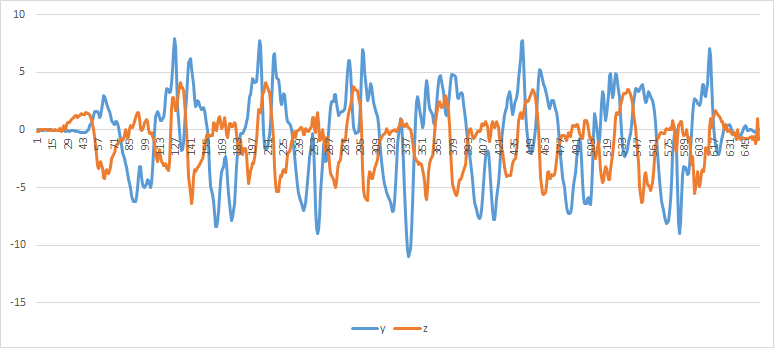
\includegraphics[scale=0.6]{imagenes/grafico_rapido.png}
	\caption{Datos del acelerómetro al realizar movimiento rápidamente.\label{fig:acc_5}}
\end{figure}

Por una parte, si la prueba se desarrolla con demasiada velocidad como se observa en la figura \ref{fig:acc_5}, la aceleración inversa que siempre tiene lugar al finalizar el desplazamiento puede llegar a unirse a la aceleración del  movimiento próximo, provocando un comportamiento más complejo de clasificar, o incluso llegando a presentar fallos.

\begin{figure}[H]
	\centering
	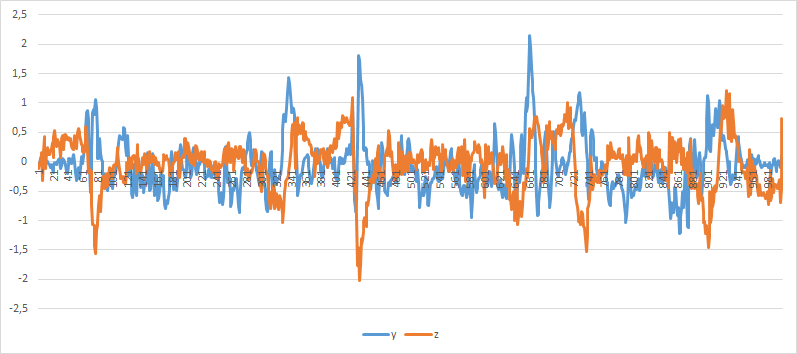
\includegraphics[scale=0.6]{imagenes/grafico_lento.png}
	\caption{Datos del acelerómetro al realizar movimiento lentamente.\label{fig:acc_6}}
\end{figure}

Por otra parte, al efectuar los desplazamientos de forma demasiado pausada (figura \ref{fig:acc_6}), los picos en los datos destacan tan poco que en ocasiones es fácil confundirlos con el propio ruido del acelerómetro, dando también lugar a fallos en algunas ocasiones. A esto hay que añadir que la precisión del sensor puede variar entre distintos dispositivos.

La mejor forma de solucionar estas adversidades sería, a falta de hacer un análisis más profundo, crear un clasificador que determine por sí mismo a qué estado se asemeja más cada patrón de datos. Sin embargo, debido a que la complejidad se escaparía de los objetivos marcados para este proyecto y también a la ausencia de \textit{datasets} suficientemente amplios con datos de acelerómetros atados al pecho durante la ejecución de esta prueba, nos hemos visto obligados a optar por el desarrollo de un algoritmo más convencional y que se desenvuelva de forma aceptable respecto a nuestros requisitos.

El funcionamiento consiste básicamente en pedir al usuario de forma ordenada que se levante y se vuelva a sentar dos veces, de forma que se miden los valores que registra el acelerómetro, se calcula la media y se guardan. Posteriormente, el usuario es libre de levantarse y sentarse hasta alcanzar las cinco repeticiones exigidas por la prueba. 

Para realizarla, se ha de empezar desde la posición sentado tanto por ser un requisito propio del test como por facilitar la medición. Cuando comience a levantarse, si supera las marcas guardadas en los ejes Z e Y durante el calibrado, se determina que se ha levantado una vez. De igual forma se procede para detectar cuándo se ha sentado el usuario.

En la práctica, el algoritmo es ligeramente más complejo ya que tiene en cuenta cuándo se inicia el movimiento y cuándo se detiene. También se reducen las marcas a superar ya que es de esperar que no siempre se acometa con la misma velocidad, a lo que se suma un tiempo de espera pequeño tras cada cambio de posición ayudando a descartar por ejemplo la aceleración producida por un rebote al sentarse bruscamente en la silla. Como el orden siempre ha de ser el mismo (sentado, levantado, sentado, etc.), no es necesario calcular completamente en qué postura se encuentra el usuario en todo momento, sino más bien determinar si ha pasado a la siguiente posición o no. No obstante eso no es suficiente para evitar errores de medición en la totalidad de casos.

Debido a la dificultad de solventar estos problemas completamente, se decidió añadir la opción de realizar la prueba con el dispositivo en el muslo. La gran diferencia es que cuando nos sentamos, el eje Y se encuentra en posición horizontal y al levantarnos, en vertical, lo cual facilita mucho la medición y reduce enormemente la posibilidad de obtener fallos independientemente de la velocidad a la que se realice u otros factores. Puede apreciarse mejor en la siguiente figura (\ref{fig:acc_muslo}), donde se representa la fuerza de la gravedad sobre el eje Y:

Cuando estamos sentados, la gráfica muestra una fuerza de gravedad cercana a cero en el eje Y, lo cual tiene sentido respecto a la organización de los ejes de coordenadas en la imagen \ref{fig:ejes_acc} del apartado \ref{sec:acc}.

En cambio, al estar de pie toda la fuerza de la gravedad recae sobre dicho eje, haciendo que su valor alcance unas cotas cercanas a uno mientras se mantenga en esa posición. Que los números sean positivos o negativos indica únicamente si el teléfono se encuentra con la parte superior hacia arriba o hacia abajo, lo cual es irrelevante para la prueba y puede ser descartado trabajando con el valor absoluto.

\begin{figure}[H]
	\centering
	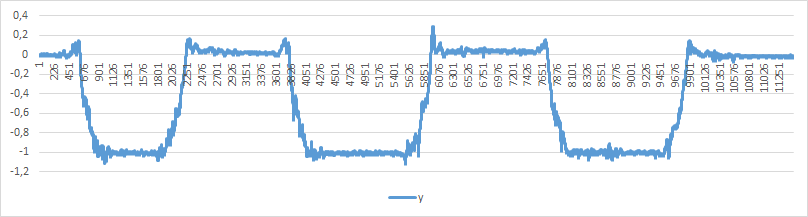
\includegraphics[scale=0.6]{imagenes/grafico_y_muslo.png}
	\caption{Datos del acelerómetro en el muslo.\label{fig:acc_muslo}}
\end{figure}

\section{Test de equilibrio}

El algoritmo desarrollado para la medición de este test es relativamente simple. Se sustenta en el hecho de que mientras se está manteniendo el equilibrio, los datos obtenidos por los tres ejes del acelerómetro deberían permanecer más o menos constantes. 

Lo que se hace es pedir al usuario que se sitúe en la posición origen (de pie, con los pies juntos) con el dispositivo en el pecho y se mantenga inmóvil hasta finalizar el calibrado. Dicho calibrado consiste básicamente en guardar los datos de todos los eje de coordenadas que devuelve el acelerómetro y hacer la media de cada uno de ellos durante unos cuantos segundos. En la gráfica de la siguiente imagen (figura \ref{fig:acc_7}) se ha mantenido el equilibrio hasta aproximadamente la mitad de la prueba, donde se aprecia de forma clara un despunte por encima de lo habitual en cualquiera de los ejes. Esto demuestra que en principio es fácil determinar el fin del test.

\begin{figure}[H]
	\centering
	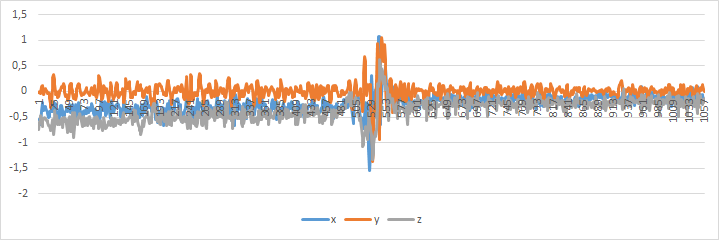
\includegraphics[scale=0.65]{imagenes/grafico_equilibrio.png}
	\caption{Datos del acelerómetro al romper equilibrio.\label{fig:acc_7}}
\end{figure}

Una vez iniciado el test, si la medición en alguno de los tres ejes excede significativamente la media calculada durante su calibración, se establece que el usuario se ha movido, se calcula la puntuación en base al tiempo transcurrido y se finaliza la prueba.

\begin{lstlisting}[language=Java]
if (calibrated && inProgress) {
    // How much the current value changes with respect to the average or
    // normal position.
    float change_x, change_y, change_z;
    change_x = Math.abs(x - mean_x);
    change_y = Math.abs(y - mean_y);
    change_z = Math.abs(z - mean_z);

    long elapsedMillis = SystemClock.elapsedRealtime() - chronometer.getBase();

    if(change_x > move_allowed || change_z > move_allowed || change_y > 1) {
        desbalanced(elapsedMillis);

    } else if (elapsedMillis > 10100) {
        chronometer.stop();
        iv_person.setImageResource(R.drawable.ic_test_done);
        continueTest();
    }
}
\end{lstlisting}

Como vemos en la línea 14 del código superior, al superar los 10.000 milisegundos (10 segundos), se finaliza la prueba y se llama a los métodos correspondientes para indicárselo al usuario y continuar con el test.

\section{Test de velocidad de marcha}

En este test nos hemos centrado en crear un algoritmo que determine el tiempo que el usuario se está moviendo. Hemos descartado para ello llevar la cuenta de los pasos dados o cualquier otro dato que dificultase la medición.

La única información utilizada ha sido la proporcionada por el eje Y. En la siguiente figura (número \ref{fig:acc_8}) vemos un patrón sencillo en el que cada despunte del gráfico equivale a un paso del usuario. Para obtener estos datos se estaba utilizando también el giroscopio, un sensor que no muchos móviles de gama baja incorporan, con lo que se optó por prescindir de él y reemplazar la información utilizando exclusivamente el acelerómetro. Aunque en la gráfica parece muy fácil determinar los pasos, la tarea se puede volver más compleja si el usuario tiene una movilidad limitada y camina muy lento o de forma muy suave.

\begin{figure}[H]
	\centering
	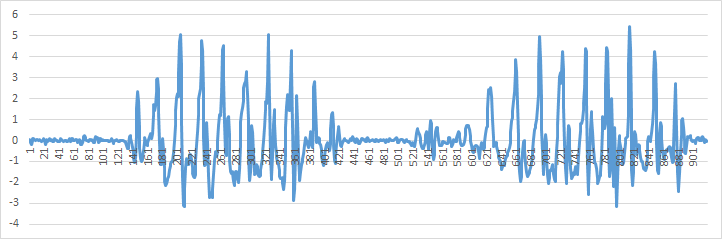
\includegraphics[scale=0.65]{imagenes/grafico_andar.png}
	\caption{Datos del acelerómetro al andar.\label{fig:acc_8}}
\end{figure}

El funcionamiento del algoritmo es el siguiente. Una vez iniciada la prueba, se empieza a contar el tiempo transcurrido y se almacena el máximo valor del eje Y obtenido hasta el momento. Con cada paso, este valor puede actualizarse si supera el máximo anterior. En caso de no superarse, si la aceleración en el eje Y es al menos mayor que un tercio del máximo registrado, se determina que el usuario está aún caminando. Cuando no se supere este valor durante un tiempo determinado (dos segundos en este caso), se señala el fin de la prueba y se calcula el tiempo total que el usuario ha estado caminando.

\begin{lstlisting}[language=Java]
if (yChange > max_change/3f){
    lastChangeTime = curTime;
    if(yChange > max_change) {
        max_change = yChange;
    }
}
\end{lstlisting}

\section{Lista de usuarios}

La lista de usuarios que aparece en la sección \textit{Usuarios} (figura \ref{fig:capturas_usuarios}) se creó en un primer momento utilizando un componente de Android denominado \textbf{ListView}. Lo que hace ListView es leer una serie de elementos (que en este caso son los usuarios guardados en la base de datos local) y mostrarlos en una lista desplazable, utilizando para ello un \textit{adaptador}. Sin embargo, se trata de un elemento algo antiguo y el funcionamiento era lento y presentaba tirones a pesar del pequeño número de usuarios que estaba mostrando. 

Por ello, se decidió sustituir ListView por el más reciente \textbf{RecyclerView}, otro componente con un objetivo prácticamente idéntico pero con un funcionamiento subyacente diferente. Mientras que ListView genera una vista nueva para cada uno de los elementos mostrados, Recyclerview reutiliza las vistas creadas para otros elementos no visibles, lo que resulta en un menor gasto de recursos y un funcionamiento más suave.

Se añadió también la posibilidad de eliminar cualquiera de los usuarios almacenados mediante un gesto llamado \textit{Swipe} o Deslizar, gesto que pudo conseguirse implementando la clase RecyclerUserTouchHelper. Al arrastrar el usuario a eliminar, se descubre un fondo rojo con un icono de papelera y un texto que indica la acción a acometer. Normalmente este fondo se crea en el momento de arrastrar ya que así se pueden añadir funciones diferentes en función de la dirección en la que se realice, sin embargo optamos por la idea de diseñar el fondo directamente en el archivo de interfaz de los objetos de lista ya que presentaba menos errores que la otra opción.

Por último, se han implementado acciones para responder tanto a un click largo sobre alguno de los usuarios almacenados, que lo señala y guarda como seleccionado (o deseleccionado si ya lo estaba), y un click o toque corto, que abre el fragmento de puntuación y lo actualiza con toda la información rescatada de la base de datos respecto al ID de usuario clicado. Estas acciones en conjunto ofrecen un comportamiento mucho más dinámico de la lista además de añadir utilidad real que mejora y amplía la experiencia de usuario.

Para guardar un usuario, al presionar el botón dedicado a tal fin y rellenar el cuadro de diálogo que aparece, se ejecutan las siguientes acciones que permiten insertar los datos obtenidos en la base de datos. Como podemos ver en la línea 3, se crea un objeto usuario a través de su constructor siendo necesario únicamente insertar el nombre que tendrá, el cual ha sido comprobado anteriormente para evitar guardar una cadena vacía. Una vez creado el objeto, se introduce en la base de datos a través del método \textit{insert} de la línea 4, que será desglosado también a continuación. También se hace en este paso la acción de marcar como seleccionado el usuario recién creado entre las líneas 6 y 8. Por último, se actualiza el componente Recyclerview para que muestre el nuevo objeto.


\begin{lstlisting}
String userName = edt.getText().toString();
if (userName.length() != 0) {
    User user = new User(edt.getText().toString());
    user.insert(getActivity());

    selectedId = user.getId();
    editor.putLong(SELECTED_USER, selectedId);
    editor.apply();

    showUsersList();
}
\end{lstlisting}

El método \textit{insert} de la clase \textit{User} que hemos comentado anteriormente lleva a cabo las siguientes acciones. En primer lugar guarda las variables del objeto en cada uno de los campos correspondientes para su almacenado (líneas 3-8). Posteriormente, crea un objeto de la clase \textit{LocalSQLiteOpenHelper} para acceder a la base de datos, obtiene ``permisos'' de escritura e inserta los valores anteriores en la tabla correspondiente. En último lugar (línea 14) nos aseguramos de cerrar el acceso a la base de datos.

\begin{lstlisting}
public void insert(Context context) {
    ContentValues values = new ContentValues();
    values.put(UsersDB.UserEntry.NAME,this.name);
    values.put(UsersDB.UserEntry.BALANCE_SCORE, this.balanceScore);
    values.put(UsersDB.UserEntry.SPEED_SCORE, this.speedScore);
    values.put(UsersDB.UserEntry.CHAIR_SCORE, this.chairScore);
    values.put(UsersDB.UserEntry.TEST_DATE, this.testDate);
    values.put(UsersDB.UserEntry.AVERAGE_SPEED, this.averageSpeed);

    LocalSQLiteOpenHelper helper = new
            LocalSQLiteOpenHelper(context);
    SQLiteDatabase db = helper.getWritableDatabase();
    this.id=db.insert("USERS", null, values);
    db.close();
}
\end{lstlisting}

El funcionamiento de los métodos utilizados para actualizar la información de algún usuario o para eliminarlo es similar al que acabamos de ver, con lo que no los comentaremos. 

\section{Pantalla de puntuación}

En la figura \ref{fig:capturas_puntuacion} vemos la pantalla de puntuación. Queríamos crear un entorno para mostrar los resultados del usuario que fuese bonito y dinámico, pero a la misma vez limpio y fácil de entender. Para ello, optamos por añadir como primer elemento un círculo que se rellenase con colores en función de la puntuación total alcanzada, a parte de mostrarla en su interior para evitar dudas. 

Este círculo se realizó usando un componente de Android denominado \textbf{ProgressBar}, muy habitual en las pantallas de carga para representar la progresión de las mismas. En nuestro caso el uso era distinto pero se adaptaba igual de bien. Utilizamos elementos XML para cambiar la apariencia y el color de la progresión. También añadimos una animación tanto al progreso de la barra como al del texto para que simulase ser un contador analógico mediante el uso de las clases ValueAnimator y ObjetAnimator.

\begin{lstlisting}
ValueAnimator animator = new ValueAnimator();
animator.setObjectValues(0, score);
animator.addUpdateListener(new ValueAnimator.AnimatorUpdateListener() {
    public void onAnimationUpdate(ValueAnimator animation) {
        tv_score.setText(String.valueOf(animation.getAnimatedValue()));
    }
});
animator.setDuration(2000); 
animator.start();

ObjectAnimator animation = ObjectAnimator.ofInt(progressBar, "progress", pb_score);
animation.setDuration(2000);
animation.setInterpolator(new DecelerateInterpolator());
animation.start();
\end{lstlisting}

Los siguientes elementos de la pantalla de puntuación son estáticos, aunque también se muestran u ocultan en función de las pruebas realizadas por el usuario. Se trata del desglose de la puntuación entre las tres pruebas, cuyo diseño ya analizamos en el capítulo correspondiente.

También aparece aquí un botón que permite salvar la información de los resultados en un usuario determinado, según haya sido seleccionado de forma previa, en caso de que la pantalla de puntuación se muestre tras finalizar un test y no al acceder desde la lista de Usuarios. Para guardar dicha información, se accede a el objeto de la clase Usuario (mUser) seleccionado y se establece la puntuación de cada una de las pruebas realizadas. En último lugar, se hace una llamada a su método \textit{update} el cual se encarga del proceso necesario para insertar la información en la base de datos.

\begin{lstlisting}
if (tv_balance_score.getVisibility() == View.VISIBLE)
    mUser.setBalanceScore(mBalanceScore);
if (tv_gait_score.getVisibility() == View.VISIBLE){
    mUser.setSpeedScore(mGaitScore);
    mUser.setAverageSpeed(mAverageSpeed);
}
if (tv_chair_score.getVisibility() == View.VISIBLE)
    mUser.setChairScore(mChairScore);
mUser.update(getActivity());
\end{lstlisting}

\section{Internacionalización y accesibilidad}

\subsection{Internacionalización}

Todos los recursos de texto que se muestran en la aplicación se encuentran agrupados en un único archivo denominado \textbf{strings.xml}, que abarca tanto títulos como descripciones e instrucciones de voz. Esto permite modificarlos de forma sencilla y rápida, a parte de poder crear archivos paralelos para ser traducidos con el objetivo de que la aplicación se adapte al idioma del mayor número de personas posible.

En la actualidad cuenta con soporte para los idiomas inglés y español de forma automática. Es decir, el lenguaje establecido por defecto en cada dispositivo afectará al lenguaje en el que se muestre la aplicación. Para añadir nuevos idiomas bastará con generar una copia traducida del archivo Strings más reciente. Se ha evitado la inclusión de texto en cualquier imagen para agilizar el proceso de internacionalización, evitando la edición pormenorizada de cada una. 

Además se ha tenido en cuenta a los idiomas con escritura de derecha a izquierda (o RTL por sus siglas en inglés), de forma que el texto adapte correctamente los márgenes y espacios en función a la dirección del mismo. Con la vista puesta en un posible lanzamiento futuro de la aplicación en mercados con esas características, se ahorrará la necesidad de editar el diseño de las múltiples interfaces a posteriori.

\subsection{Accesibilidad}

La aplicación adapta la mayoría de los textos a las preferencias de tamaño establecidas por el usuario. Esto es realmente útil y muy importante en especial para la población anciana, que suele establecer el máximo tamaño de fuente debido a problemas de visión. Además, se ha estudiado el comportamiento de todas las secciones para asegurar que el cambio de tamaño no impide la correcta visualización de los elementos, añadiendo la posibilidad de realizar deslizamientos en aquellas pantallas donde el texto pueda exceder los límites de la misma. 

Por otra parte, también se ha tenido en cuenta el funcionamiento de herramientas de accesibilidad como Talkback, así que todas las imágenes y botones sin texto que requieren de una explicación en caso de no poder ser visualizados tienen su correspondiente descripción en todos los idiomas en los que la app está disponible.

\section{Miscelánea}

Aquí listaremos otras características importantes para el correcto funcionamiento de la aplicación pero que no se muestran a simple vista en la mayoría de casos.

\subsection{Carencia de acelerómetro}

El funcionamiento de todo este proyecto está orientado a la realización del test mediante el sensor acelerómetro de los teléfonos. En caso de que algún dispositivo no cuente con él, pueden presentarse fallos y cierres inesperados si no se trata de forma correcta. 

Por este motivo se decidió mostrar un mensaje al abrir la aplicación en esos casos en los que el móvil no posea el sensor necesario, indicando al usuario la razón por la que la aplicación no puede ser usada. Puede verse en la figura siguiente (\ref{fig:no_acc}).

\begin{figure}[H]
	\centering
	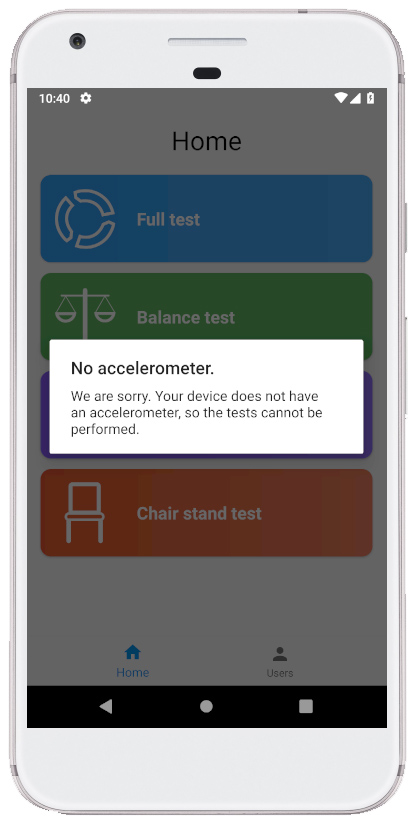
\includegraphics[scale=0.35]{imagenes/no_acc.jpg}
	\caption{No hay acelerómetro.\label{fig:no_acc}}
\end{figure}

\subsection{Posición fija de pantalla}

Debido a que durante la realización del test SPPB el móvil deberá permanecer sujeto al pecho y en una posición concreta (vertical), no tiene sentido que al girar el teléfono la pantalla también gire, provocando además una visualización incorrecta de la interfaz y problemas en la medición. Por esta razón, se ha determinado que todas los fragmentos que aparecen dentro de la actividad TestActivity (\ref{fig:navegacion}) estén fijos en posición vertical, independientemente de la orientación del teléfono. El resto de actividades y fragmentos sí que pueden girar y adaptarse.

\subsection{Evitar bloqueo durante test}
La mayoría de usuarios establece un tiempo tras el cual la pantalla se apaga y el dispositivo se bloquea. Aunque es una buena forma de ahorrar batería, pero que esto suceda durante la ejecución de las pruebas puede dar como resultado la incompletitud de las mismas o todo tipo de fallos.

Para subsanar este problema, se añadió la característica de que la pantalla nunca se apague mientras se encuentre dentro de la actividad TestActivity (\ref{fig:navegacion}), lo que implica que el móvil siempre está activo durante la realización de cualquiera de los tests. Al abandonar dicha actividad, se desactiva esta herramienta y la pantalla recupera su comportamiento habitual.



\chapter{Pruebas}

\section{Teléfonos utilizados}

Para comprobar y asegurar el correcto funcionamiento de la aplicación en el mayor número de casos posibles, hemos utilizado diferentes dispositivos móviles con características dispares de software, tamaño de pantalla, densidad de píxeles o tamaño de fuente, entre otras.

En concreto, los teléfonos utilizados han sido:

\begin{table}[H]
\centering
\begin{tabular}{|l|l|l|l|l}
\cline{1-4}
\textbf{Marca} & \textbf{Modelo} & \textbf{Versión de software} & \textbf{Pantalla} & \\ \cline{1-4}
    Google & Pixel XL & API 28 (Android 9 Pie) & 5,5" &  \\ \cline{1-4}
    Google & Pixel XL & API 29 (Android 10) & 5,5" &  \\ \cline{1-4}
    Huawei & ALE-L21 & API 23 (Android 6.0 Marshmallow) & 5" &  \\ \cline{1-4}
    Xiaomi & Mi A2 Lite & API 28 (Android 9 Pie) & 5,84", notch &  \\ \cline{1-4}
    Nexus  & 5 & API 21 (Android 5 Lollipop) & 4,95" &  \\ \cline{1-4}
    ZTE  & BLADE A512 & API 23 (Android 5 Lollipop) & 5,2" &  \\ \cline{1-4}
\end{tabular}
\end{table}

No todos los teléfonos tienen además la misma forma de pantalla. Es el caso del Xiaomi Mi A2 Lite, cuya pantalla es bastante más alargada y menos ancha que la del resto de dispositivos. 

Por otra parte, tanto el Xiaomi recién mencionado como el Huawei ALE-L21 son utilizados con el máximo tamaño de texto permitido. En el caso del ZTE BLADE, la resolución de pantalla (densidad de píxeles) no es muy alta, lo que provoca que todos los elementos aparezcan con una mayor dimensión. Tener estos datos en cuenta es importante para comprobar que el diseño de la interfaz no se desorganiza, provocando solapamientos en las cadenas de texto o desbordamientos fuera de pantalla que impedirían la correcta visualización de información. 

Salvo los problemas que comentaremos en el siguiente apartado, todo funciona correctamente en cada uno los móviles de la tabla superior, asegurando el correcto funcionamiento del proyecto en un bastante amplio rango de dispositivos.

\section{Problemas en otros dispositivos}

\subsection{Visualización incorrecta de algunas imágenes}

En algunas versiones de Android con una API inferior a 23, se presentaba un extraño error que provocaba la incorrecta visualización de imágenes vectoriales, imágenes que sí se veían correctamente en el resto de dispositivos.

Parece ser un fallo más o menos común. Tras distintos intentos, la única forma de solucionarlo ha sido sustituir las imágenes vectoriales afectadas por su versión en formato PNG, el cual muestra las imágenes tal y como fueron diseñadas. La contrapartida de esta decisión es que el tamaño de los recursos PNG es muy superior al de los vectoriales, a lo que hay que añadir la necesidad en Android de incorporar múltiples versiones de la misma imagen con distintas resoluciones para evitar que pierdan calidad en pantallas más grandes.

\begin{figure}[H]
	\centering
	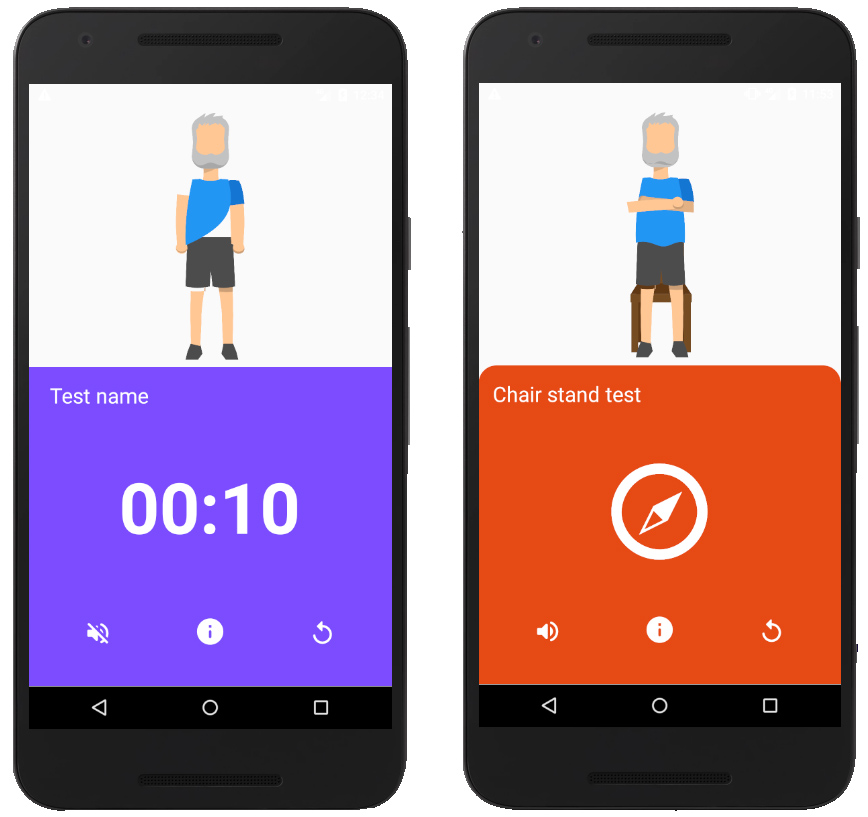
\includegraphics[scale=0.30]{imagenes/errores.jpg}
	\caption{Errores de visualización vectorial.\label{fig:errores}}
\end{figure}

\subsection{Periodos de muestreo diferentes}

El periodo o frecuencia de muestreo es el tiempo que transcurre entre que el servicio de acelerómetro ofrece un dato y el siguiente. 

Durante el desarrollo de la aplicación se había establecido un periodo de muestreo de 1Hz, es decir, se pretendía obtener los datos del acelerómetro cada 1 segundo. Sin embargo, esta frecuencia no se cumplía de igual forma en todos los dispositivos de la tabla anterior, lo que provocó que mientras la evaluación de las pruebas se llevaba a cabo de forma correcta en el teléfono de desarrollo (Google Pixel XL), el funcionamiento fuese totalmente impredecible en otros.

Veamos algunos comportamientos concretos. En el teléfono Xiaomi Mi A2 Lite la tasa de muestreo estaba siendo muy superior a la establecida, llegando a devolver la aceleración que se conseguía cada pocas milésimas de segundo. Como es de imaginar, la aceleración acumulada que se produce entre dos espacios de tiempo muy cercanos será menor que la que se produce entre dos espacios de tiempo separados por un segundo. Esta aceleración, al ser tan pequeña, es muy fácil de igualar incluso sin moverse (como resultado del ruido en los datos), lo que convertía la prueba de levantarse y sentarse en la silla en un conjunto de errores sin la más mínima fiabilidad puesto que constantemente determinaba que el usuario se había levantado y sentado.

Por otra parte, el teléfono Huawei ALE-L21 tenía un periodo de muestreo muy lento, lo que impedía por completo el funcionamiento de las tres pruebas. 

Finalmente, el problema se resolvió estableciendo una tasa de refresco por defecto (\textit{sensor\_delay\_game}) en todos los tests, y controlando mediante un condicional \textit{if} que no se accede a la información del acelerómetro hasta que no ha transcurrido un tiempo mínimo de 100 milisegundos. 

\begin{lstlisting}
sensorManager.registerListener(this, sensorAcc, SensorManager.SENSOR_DELAY_GAME);
\\ ...
if ((System.currentTimeMillis() - lastSaved) > ACCE_FILTER_DATA_MIN_TIME) {
    \\ ... 
}
\end{lstlisting}

\subsection{Falta de soporte de características visuales}

En las versiones de software más bajas soportadas por la aplicación, hay determinados elementos estéticos que no pueden visualizarse por falta de soporte. Un ejemplo es el color personalizado de la barra de estado para dispositivos con API 21, que se utiliza en toda la aplicación para mostrarla del mismo color blanco que el fondo, o de una tonalidad más oscura del color correspondiente en la actividad de instrucciones.

\section{Pruebas en usuarios}

Se han llevado a cabo pruebas sobre usuarios reales para la persecución de múltiples objetivos. 

Por una parte, durante la evolución individual de cada uno de los algoritmos de medición, era necesario poner a prueba continuamente los avances en el proyecto, tarea que ha recaído principalmente sobre el desarrollador. A medida que estos algoritmos abandonaban el estado de desarrollo para acercarse al de producción, han sido otros usuarios con diferentes edades (comprendidas entre los 20 y los 60 años) los que han participado en las pruebas.

Se les ha pedido usar la aplicación de forma autónoma, una actividad muy útil de cara a estudiar, por ejemplo, dificultades entendiendo el funcionamiento de la interfaz.

\begin{figure}[H]
	\centering
	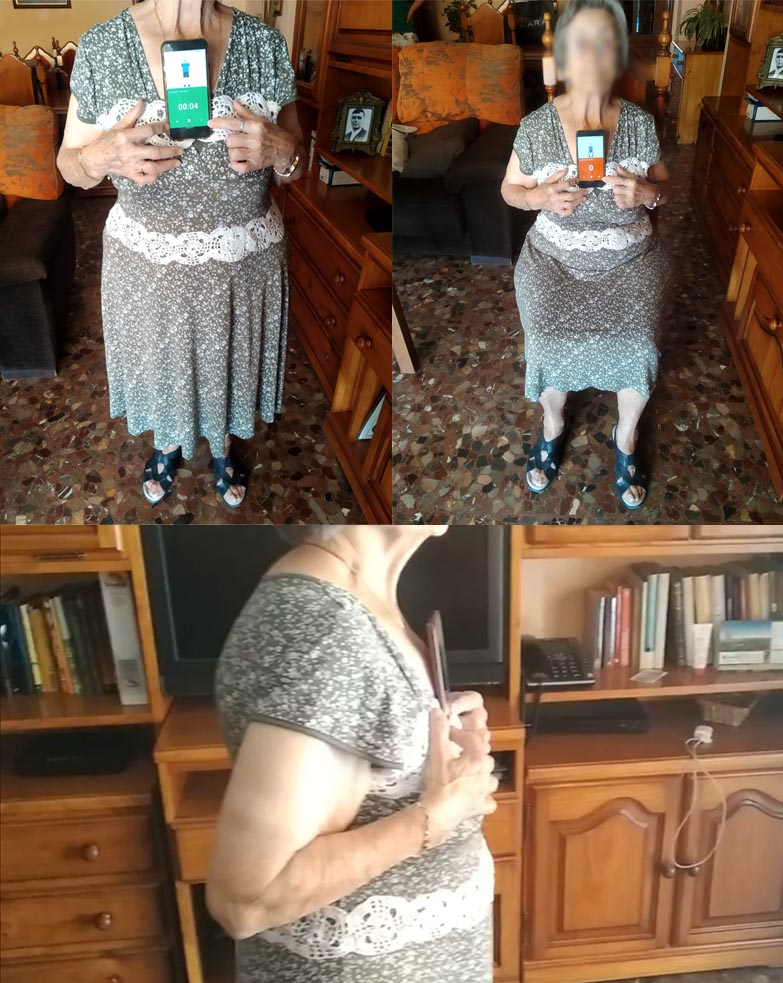
\includegraphics[scale=1.5]{imagenes/pruebas.jpg}
	\caption{Pruebas con ancianos.\label{fig:pruebas_mayores}}
\end{figure}

A medida que se localizaban errores durante la utilización con usuarios reales, se tomaban medidas para corregirlos o adaptarlos. De este modo se han pulido diversos aspectos de la aplicación hasta alcanzar un estado apto para pruebas con personas más mayores (más de 85 años) como se puede ver en la figura superior \ref{fig:pruebas_mayores}.

En general, los resultados obtenidos mediante las pruebas llevadas a cabo en las últimas fases del desarrollo de la \textit{app} han sido satisfactorios. Los usuarios comprendían de forma aceptable cómo navegar por la interfaz y las instrucciones para la realización de los tests. Además, las mediciones eran correctas en la mayoría de casos a excepción del test de \textit{levantarse de la silla con el móvil en el pecho}, el cual deberá sufrir aún más mejoras.

Estas pruebas no se han empleado para ningún propósito más allá del de mejorar y enriquecer el proyecto. Por tanto, no nos hemos ocupado de crear estadísticas de errores surgidos tanto en la ejecución como en el manejo de la aplicación.

Se espera, no obstante, una colaboración con el Departamento de Enfermería y Fisioterapia de la Universidad de Cádiz y con el Institute of Artificial Intelligence de De Montfort University en Leicester (Reino Unido) para validar los resultados con más usuarios reales durante los próximos meses.


\chapter{Conclusiones y trabajo futuro}

\section{Conclusiones}

Llegamos al término de este proyecto. El tiempo invertido durante estos meses de trabajo nos ha conducido a nuevos conocimientos en varios ámbitos. 

Por una parte, ahora sabemos de los peligros de la fragilidad que afecta a un gran número de ancianos. Conocemos las estimaciones de crecimiento de esta parte de la población y la importancia de tomar decisiones a tiempo en el campo de la salud. Hemos hablado sobre los aportes del test Guralnikj, en qué consiste y cómo es capaz de determinar con bastante acierto la presencia fragilidad en las personas. También hemos visto que sus resultados son muy aceptados en la medicina, algunos de los lugares donde se aplica e instituciones que aconsejan su empleo.

Por otra parte, nos hemos enfrentado a la creación y el desarrollo de una aplicación para Android contando previamente con una experiencia muy pobre en el mundo de los dispositivos móviles. Hemos trabajado con los sensores del dispositivo, analizado e integrado sus resultados, automatizado el almacenamiento de los mismos mediante la creación de una base de datos local y cubierto el código bajo una bonita interfaz. Todo esto ha sido gracias a las distintas enseñanzas y disciplinas cursadas durante la carrera, donde sobre todo han conseguido ilustrarnos en la búsqueda de soluciones de forma ágil y autónoma.

Finalmente podemos presentar un resultado que cumple con los requisitos que habíamos establecido y los tiempos dados. Una aplicación que permite realizar el test SPPB sin necesidad de ninguna herramienta adicional al móvil y que integra varias disciplinas. Además nos hemos iniciado en la documentación de proyectos, aprendiendo a estructurar el contenido de forma clara y desarrollar nuestras ideas para que sean legibles.

\section{Trabajos futuros}

Por fortuna, son muchas las funcionalidades que se nos han ido ocurriendo y que aún podríamos implementar para mejorar y ampliar la utilidad de este proyecto. Algunas de las más destacables son estas:

\begin{itemize}
    \item \textbf{Mostrar ejercicios recomendados y hábitos de vida saludable} en función de la puntuación obtenida. Además, podría incorporarse una nueva pestaña en la que periódicamente se publiquen recomendaciones y estudios médicos que puedan ser de utilidad a los mayores. 
    
    \item \textbf{Guardar los resultados de las pruebas anteriores}, poder navegar entre ellas y mostrar con un gráfico la evolución de cada usuario. Además podría señalarse especialmente aquellos casos en los que se obtenga un peor resultado que en ocasiones anteriores y tomar medidas como sugerir actividades complementarias para tratar de paliar esta situación.
    
    \item \textbf{Añadir nuevos tests} que ayuden a evaluar sintomatologías diferentes. De este modo, ampliaríamos la aplicación integrando más funciones que evitarían el uso de herramientas específicas.
    
    \item \textbf{Mejorar la precisión de medición en algunas de las pruebas} e incorporar clasificadores entrenados con big data para analizar y evaluar la ejecución de las mismas.
    
    \item \textbf{Llevar un registro de las actividades realizadas por el usuario} como caminar, subir escaleras, etc. y enviarle una notificación cuando no las cumpla.
    
    \item \textbf{Permitir crear o seleccionar usuarios distintos} en la pantalla de puntuación. Así se flexibilizará y facilitará el guardado de datos.
\end{itemize}

Además, como hemos mencionado anteriormente, la aplicación será validada con \textbf{usuarios reales} en colaboración con el \textbf{Departamiento de Enfermería y Fisioterapia de la Universidad de Cádiz} y con el \textbf{Institute of Artificial Intelligence de De Montfort University, Leicester UK.}


%%\nocite{*}
%\bibliography{bibliografia/bibliografia}\addcontentsline{toc}{chapter}{Bibliografía}
%\bibliographystyle{miunsrturl}
\bibliography{bibliografia/bibliografia}
\addcontentsline{toc}{chapter}{Bibliografía}
\bibliographystyle{plain}

\appendix
\chapter{Manual de usuario}

\includepdf[pages=-]{apendices/manual_usuario/Manual_usuario}
%%\input{apendices/paper/paper}
%\input{glosario/entradas_glosario}
% \addcontentsline{toc}{chapter}{Glosario}
% \printglossary
\chapter*{}
\thispagestyle{empty}

\end{document}
